\documentclass{amsart}
% !TEX root = ../cobar1.tex

\usepackage{microtype}
\usepackage{amssymb}
\usepackage{mathtools}
\usepackage{tikz-cd}
\usepackage{mathbbol} % changes \mathbb{} and adds more support

% bibliography
\usepackage[
	backend=biber,
	style=alphabetic,
	backref=true,
	url=false,
	doi=false,
	isbn=false,
	eprint=false]{biblatex}

\renewbibmacro{in:}{}  % don't display "in:" before the journal name
\AtEveryBibitem{\clearfield{pages}}  % don't show page numbers

\DeclareFieldFormat{title}{\myhref{\mkbibemph{#1}}}
\DeclareFieldFormat
[article,inbook,incollection,inproceedings,patent,thesis,unpublished]
{title}{\myhref{\mkbibquote{#1\isdot}}}

\newcommand{\doiorurl}{%
	\iffieldundef{url}
	{\iffieldundef{eprint}
		{}
		{http://arxiv.org/abs/\strfield{eprint}}}
	{\strfield{url}}%
}

\newcommand{\myhref}[1]{%
	\ifboolexpr{%
		test {\ifhyperref}
		and
		not test {\iftoggle{bbx:eprint}}
		and
		not test {\iftoggle{bbx:url}}
	}
	{\href{\doiorurl}{#1}}
	{#1}%
}

% references
\usepackage[
	bookmarks=true,
	linktocpage=true,
	bookmarksnumbered=true,
	breaklinks=true,
	pdfstartview=FitH,
	hyperfigures=false,
	plainpages=false,
	naturalnames=true,
	colorlinks=true,
	pagebackref=false,
	pdfpagelabels]{hyperref}

\hypersetup{
	colorlinks,
	citecolor=blue,
	filecolor=blue,
	linkcolor=blue,
	urlcolor=blue
}

\usepackage[capitalize, noabbrev]{cleveref}
\let\subsectionSymbol\S
\crefname{subsection}{\subsectionSymbol\!\!}{subsections}

% layout
\addtolength{\textwidth}{0in}
\addtolength{\textheight}{0in}
\calclayout

% update to MSC2020
\makeatletter
\@namedef{subjclassname@2020}{%
	\textup{2020} Mathematics Subject Classification}
\makeatother

% table of contents
\setcounter{tocdepth}{4}

% environments
\newtheorem{theorem}{Theorem}
\newtheorem{proposition}[theorem]{Proposition}
\newtheorem{lemma}[theorem]{Lemma}
\newtheorem{corollary}[theorem]{Corollary}
\theoremstyle{definition}
\newtheorem{definition}[theorem]{Definition}
\newtheorem{example}[theorem]{Example}
\newtheorem{remark}[theorem]{Remark}

% hyphenation
\hyphenation{co-chain}

% elements
\newcommand{\id}{\mathsf{id}}
\newcommand{\M}{\cM}
\newcommand{\UM}{{\forget(\M)}}
\newcommand{\SL}{{\M_{sl}}}
\newcommand{\USL}{{\forget(\M_{sl})}}
\newcommand{\Surj}{\cX}
\newcommand{\BE}{\cE}

% sets and spaces
\newcommand{\N}{\mathbb{N}}
\newcommand{\Z}{\mathbb{Z}}
\newcommand{\R}{\mathbb{R}}
\renewcommand{\k}{\Bbbk}
\renewcommand{\S}{\mathbb{S}}
\newcommand{\Fp}{{\mathbb{F}_p}}
\newcommand{\Cp}{{\mathrm{C}_p}}
\newcommand{\graphs}{\mathfrak{G}}
\newcommand{\gsimplex}{\mathbb{\Delta}}
\newcommand{\gcube}{\mathbb{I}}

% categories
\newcommand{\Cat}{\mathsf{Cat}}
\newcommand{\Fun}{\mathsf{Fun}}
\newcommand{\Set}{\mathsf{Set}}
\newcommand{\Top}{\mathsf{Top}}
\newcommand{\Ch}{\mathsf{Ch}}
\newcommand{\simplex}{\triangle}
\newcommand{\sSet}{\mathsf{sSet}}
\newcommand{\cube}{\square}
\newcommand{\cSet}{\mathsf{cSet}}
\newcommand{\Alg}{\mathsf{Alg}}
\newcommand{\coAlg}{\mathsf{coAlg}}
\newcommand{\biAlg}{\mathsf{biAlg}}
\newcommand{\sGrp}{\mathsf{sGrp}}
\newcommand{\Nec}{\mathsf{Nec}}
\newcommand{\nSet}{\mathsf{nSet}}
\newcommand{\Mon}{\mathsf{Mon}}
\newcommand{\Smod}{\mathsf{Mod}_{\S}}
\newcommand{\Sbimod}{\mathsf{biMod}_{\S}}
\newcommand{\operads}{\mathsf{Oper}}
\newcommand{\props}{\mathsf{Prop}}

% operators
\DeclareMathOperator{\free}{F}
\DeclareMathOperator{\forget}{U}
\newcommand{\yoneda}{\mathcal{Y}}
\DeclareMathOperator{\chains}{N}
\DeclareMathOperator{\schains}{N^{\simplex}}
\DeclareMathOperator{\cchains}{N^{\cube}}
\DeclareMathOperator{\sSing}{Sing^{\simplex}}
\DeclareMathOperator{\cSing}{Sing^{\cube}}
\DeclareMathOperator{\loops}{\Omega}
\DeclareMathOperator{\cobar}{\mathbf{\Omega}}

% other
\renewcommand{\th}{\mathrm{th}}
\newcommand{\op}{\mathrm{op}}
\DeclareMathOperator*{\colim}{colim}
\DeclareMathOperator{\coker}{coker}
\newcommand{\tensor}{\otimes}
\newcommand{\End}{\mathrm{End}}
\newcommand{\Hom}{\mathrm{Hom}}
\newcommand{\bars}[1]{\lvert#1\rvert}
\newcommand{\norm}[1]{\lVert#1\Vert}
\newcommand{\angles}[1]{\langle#1\rangle}
\newcommand{\pairing}[2]{\langle#1, #2\rangle}
\newcommand{\xla}[1]{\xleftarrow{#1}}
\newcommand{\xra}[1]{\xrightarrow{#1}}
\newcommand{\defeq}{\stackrel{\mathrm{def}}{=}}
\newcommand{\pdfEinfty}{\texorpdfstring{${E_\infty}$}{E-infty}}

% letters
\newcommand{\sA}{\mathsf{A}}
\newcommand{\sB}{\mathsf{B}}
\newcommand{\sC}{\mathsf{C}}

\newcommand{\cA}{\mathcal{A}}
\newcommand{\cB}{\mathcal{B}}
\newcommand{\cC}{\mathcal{C}}
\newcommand{\cD}{\mathcal{D}}
\newcommand{\cE}{\mathcal{E}}

\newcommand{\cM}{\mathcal{M}}
\newcommand{\cN}{\mathcal{N}}
\newcommand{\cO}{\mathcal{O}}
\newcommand{\cP}{\mathcal{P}}

\newcommand{\cX}{\mathcal{X}}
\newcommand{\cY}{\mathcal{Y}}
\newcommand{\cZ}{\mathcal{Z}}

% comments
\newcommand{\anibal}[1]{\textcolor{blue}{\underline{Anibal}: #1}}

% !TEX root = ../cobar1.tex

\newcommand{\s}[1]{s^{\scalebox{.6}{{#1}}}}
\DeclareMathOperator{\aug}{\varepsilon}

\newcommand{\Smod}{\mathsf{Mod}_{\S}}
\newcommand{\Sbimod}{\mathsf{biMod}_{\S}}
\newcommand{\graphs}{\mathfrak{G}}
\renewcommand{\S}{\mathbb{S}}
\newcommand{\biEnd}{\mathrm{biEnd}}

\newcommand{\As}{{\mathcal{A}\mathsf{s}}}
\newcommand{\Com}{\cC{om}}
\newcommand{\M}{\cM}
\newcommand{\UM}{{\forget(\M)}}
\newcommand{\USL}{{\forget(\M_{sl})}}

\DeclareMathOperator{\adams}{A}
\DeclareMathOperator{\adamsE}{\widehat{A}}
\DeclareMathOperator{\adamsEA}{\widehat{A}_{\!\As}}
\DeclareMathOperator{\adamsEUM}{\widehat{A}_{\UM}}

\DeclareMathOperator{\schains}{N^{\simplex}}
\DeclareMathOperator{\cchains}{N^{\cube}}
\DeclareMathOperator{\scochains}{N^{\vee}_{\simplex}}
\DeclareMathOperator{\ccochains}{N^{\vee}_{\cube}}
\DeclareMathOperator{\Schains}{S}
\DeclareMathOperator{\sSchains}{S^{\simplex}}
\DeclareMathOperator{\cSchains}{S^{\cube}}
\DeclareMathOperator{\schainsA}{N^{\simplex}_{\!\As}}
\DeclareMathOperator{\cchainsA}{N^{\cube}_{\!\As}}
\DeclareMathOperator{\SchainsA}{S_{\!\As}}
\DeclareMathOperator{\sSchainsA}{S^{\simplex}_{\!\As}}
\DeclareMathOperator{\cSchainsA}{S^{\cube}_{\!\As}}
\DeclareMathOperator{\sSchainsUM}{S^{\simplex}_{\UM}}
\DeclareMathOperator{\cSchainsUM}{S^{\cube}_{\UM}}
\DeclareMathOperator{\schainsUM}{N^{\simplex}_{\UM}}
\DeclareMathOperator{\cchainsUM}{N^{\cube}_{\UM}}
\DeclareMathOperator{\schainsUSL}{N^{\simplex}_{\USL}}
\DeclareMathOperator{\cchainsUSL}{N^{\cube}_{\USL}}

\DeclareMathOperator{\sSing}{Sing^{\simplex}}
\DeclareMathOperator{\cSing}{Sing^{\cube}}

\DeclareMathOperator{\ccobar}{\mathbb{\Omega}}
\DeclareMathOperator{\ccobarE}{\widehat{\mathbb{\Omega}}}
\DeclareMathOperator{\ncobar}{\mathbb{\Omega}^{\mathrm{nec}}}
\DeclareMathOperator{\ncobarE}{\widehat{\mathbb{\Omega}}^{\mathrm{nec}}}

\DeclareMathOperator{\cartanserre}{\xi}
\DeclareMathOperator{\rigid}{\mathfrak{C}}
\DeclareMathOperator{\nerve}{\mathfrak{N}}
\DeclareMathOperator{\classifying}{\overline{W}}
\DeclareMathOperator{\localization}{\mathcal{L}}
\DeclareMathOperator{\kan}{G}
\DeclareMathOperator{\triangulate}{\mathcal{T}}

\newcommand{\Nec}{\mathsf{Nec}}
\newcommand{\nSet}{\mathsf{nSet}}

\newcommand{\manuel}[1]{\textcolor{red}{\underline{Manuel}: #1}}

\newcommand{\pdfM}{\texorpdfstring{${\cM}$}{M}} % add new commands
\addbibresource{aux/usualpapers.bib}
\addbibresource{aux/bibliography.bib} % add references
%%%%%%%%%%%%%%%%%%%%%%#

\title[Adams' cobar construction as a monoidal $E_{\infty}$-coalgebra]{Adams' cobar construction as a monoidal $E_{\infty}$-coalgebra model of the based loop space}

\author[A. Medina-Mardones]{Anibal M. Medina-Mardones}
\address{A.M-M., LAGA, Universit\'e Sorbonne Paris Nord}
\email{\href{medina-mardones@math.univ-paris13.fr}{medina-mardones@math.univ-paris13.fr}}

\author[M. Rivera]{Manuel Rivera}
\address{M.R., Department of Mathematics, Purdue University}
\email{\href{mailto:manuelr@purdue.edu}{manuelr@purdue.edu}}

\subjclass[2020]{57T30, 55P35, 18N70, 55U10, 55N45, 55S05}
\keywords{Adams' cobar construction, based loop space, ${E_\infty}$-structure}

\usetikzlibrary{arrows,decorations.markings}
\tikzset{myptr/.style={decoration={markings,mark=at position 1 with %
			{\arrow[scale=2,>=stealth]{>}}},postaction={decorate}}}
		
\newsavebox\preproduct
\begin{lrbox}{\preproduct}
	\begin{tikzpicture}[scale=.3]
	\draw (0,0)--(0,-.8);
	\draw (0,0)--(.5,.5);
	\draw (0,0)--(-.5,.5);
	\end{tikzpicture} 
\end{lrbox}
\newcommand{\product}{% <- this 'right of' is inherited; how to avoid?
	\usebox\preproduct}

\newsavebox\precoproduct
	\begin{lrbox}{\precoproduct}
		\begin{tikzpicture}[scale=.3]
		\draw (0,0)--(0,.8);
		\draw (0,0)--(.5,-.5);
		\draw (0,0)--(-.5,-.5);
		\end{tikzpicture}
	\end{lrbox}
\newcommand{\coproduct}{% <- this 'right of' is inherited; how to avoid?
	\usebox\precoproduct}

\newsavebox\preboundary
\begin{lrbox}{\preboundary}
	\begin{tikzpicture}[scale=.3]
	\draw (0,0)--(0,1.3);
	\draw (.5,0)--(.5,1.3);
	\draw [fill] (0,0) circle [radius=0.1];
	\draw (.9,.6)--(1.3,.6);
	\draw (1.7,0)--(1.7,1.3);
	\draw (2.2,0)--(2.2,1.3);
	\draw [fill] (2.2,0) circle [radius=0.1];
	\end{tikzpicture}
\end{lrbox}
\newcommand{\boundary}{% <- this 'right of' is inherited; how to avoid?
	\usebox\preboundary}

\newsavebox\preleftboundary
\begin{lrbox}{\preleftboundary}
	\begin{tikzpicture}[scale=.3]
	\draw (1.7,0)--(1.7,1.3);
	\draw (2.2,0)--(2.2,1.3);
	\draw [fill] (2.2,0) circle [radius=0.1];
	\end{tikzpicture}
\end{lrbox}
\newcommand{\leftboundary}{% <- this 'right of' is inherited; how to avoid?
	\usebox\preleftboundary}

\newsavebox\prerightboundary
\begin{lrbox}{\prerightboundary}
	\begin{tikzpicture}[scale=.3]
	\draw (0,0)--(0,1.3);
	\draw (.5,0)--(.5,1.3);
	\draw [fill] (0,0) circle [radius=0.1];
	\end{tikzpicture}
\end{lrbox}
\newcommand{\rightboundary}{% <- this 'right of' is inherited; how to avoid?
	\usebox\prerightboundary}

\newsavebox\precoboundary
\begin{lrbox}{\precoboundary}
	\begin{tikzpicture}[scale=.3]
	\draw (0,0)--(0,1.3);
	\draw (.5,0)--(.5,1.3);
	\draw [fill] (0,1.3) circle [radius=0.1];
	\draw (.9,.6)--(1.3,.6);
	\draw (1.7,0)--(1.7,1.3);
	\draw (2.2,0)--(2.2,1.3);
	\draw [fill] (2.2,1.3) circle [radius=0.1];
	\end{tikzpicture}
\end{lrbox}
\newcommand{\coboundary}{% <- this 'right of' is inherited; how to avoid?
	\usebox\precoboundary}

\newsavebox\precounit
\begin{lrbox}{\precounit}
	\begin{tikzpicture}[scale=.3]
	\draw (0,0)--(0,1.3);
	\draw [fill] (0,0) circle [radius=0.1];
	\end{tikzpicture}
\end{lrbox}
\newcommand{\counit}{% <- this 'right of' is inherited; how to avoid?
	\usebox\precounit}

\newsavebox\preidentity
\begin{lrbox}{\preidentity}
	\begin{tikzpicture}[scale=.3]
	\draw (0,0)--(0,1.3);
	\end{tikzpicture}
\end{lrbox}
\newcommand{\identity}{% <- this 'right of' is inherited; how to avoid?
	\usebox\preidentity}

\newsavebox\preunit
\begin{lrbox}{\preunit}
	\begin{tikzpicture}[scale=.3]
	\draw (0,0)--(0,1.3);
	\draw [fill] (0,1.3) circle [radius=0.1];
	\end{tikzpicture}
\end{lrbox}
\newcommand{\unit}{% <- this 'right of' is inherited; how to avoid?
	\usebox\preunit}

\newsavebox\preassociativity
\begin{lrbox}{\preassociativity}
	\begin{tikzpicture}[scale=.2]
	\path[draw] (0,0)--(0,1)--(-1,2);
	\draw (0,1)--(1,2);
	\draw (-.5,1.5)--(0,2);
	\draw (1.2,1)--(1.8,1);
	\path[draw] (3,0)--(3,1)--(2,2);
	\draw (3,1)--(4,2);
	\draw (3.5,1.5)--(3,2);	
	\end{tikzpicture}
\end{lrbox}
\newcommand{\associativity}{% <- this 'right of' is inherited; how to avoid?
	\usebox\preassociativity}

\newsavebox\precoassociativity
\begin{lrbox}{\precoassociativity}
	\begin{tikzpicture}[scale=.2]
	\path[draw] (0,0)--(0,-1)--(-1,-2);
	\draw (0,-1)--(1,-2);
	\draw (-.5,-1.5)--(0,-2);
	\draw (1.2,-1)--(1.8,-1);
	\path[draw] (3,0)--(3,-1)--(2,-2);
	\draw (3,-1)--(4,-2);
	\draw (3.5,-1.5)--(3,-2);
	\end{tikzpicture}
\end{lrbox}
\newcommand{\coassociativity}{% <- this 'right of' is inherited; how to avoid?
	\usebox\precoassociativity}

\newsavebox\preleftcomb
\begin{lrbox}{\preleftcomb}
	\begin{tikzpicture}[scale=.2]
	\path[draw] (0,0)--(0,-1)--(-1,-2);
	\draw (0,-1)--(1,-2);
	\draw (-.5,-1.5)--(0,-2);
	\end{tikzpicture}
\end{lrbox}
\newcommand{\leftcomb}{% <- this 'right of' is inherited; how to avoid?
	\usebox\preleftcomb}

\newsavebox\prerightcomb
\begin{lrbox}{\prerightcomb}
	\begin{tikzpicture}[scale=.2]
	\path[draw] (3,0)--(3,-1)--(2,-2);
	\draw (3,-1)--(4,-2);
	\draw (3.5,-1.5)--(3,-2);
	\end{tikzpicture}
\end{lrbox}
\newcommand{\rightcomb}{% <- this 'right of' is inherited; how to avoid?
	\usebox\prerightcomb}

\newsavebox\preinvolution
\begin{lrbox}{\preinvolution}
	\begin{tikzpicture}[scale=.2]
	\path[draw] (0,0)--(0,.5)--(-.5,1)--(0,1.5)--(0,2);
	\path[draw] (0,.5)--(.5,1)--(0,1.5);
	\end{tikzpicture}
\end{lrbox}
\newcommand{\involution}{% <- this 'right of' is inherited; how to avoid?
	\usebox\preinvolution}

\newsavebox\preleftcounitality
\begin{lrbox}{\preleftcounitality}
	\begin{tikzpicture}[scale=.3]
	\draw (0,0)--(0,.8);
	\draw (0,0)--(.5,-.5);
	\draw (0,0)--(-.5,-.5);
	\draw [fill] (-.5,-.5) circle [radius=0.1];
	\draw (.7,0)--(1.1,0);
	\path[draw] (1.5,-.5)--(1.5,.8);
	\end{tikzpicture}
\end{lrbox}
\newcommand{\leftcounitality}{% <- this 'right of' is inherited; how to avoid?
	\usebox\preleftcounitality}

\newsavebox\preleftcounitcoproduct
\begin{lrbox}{\preleftcounitcoproduct}
	\begin{tikzpicture}[scale=.3]
	\draw (0,0)--(0,.8);
	\draw (0,0)--(.5,-.5);
	\draw (0,0)--(-.5,-.5);
	\draw [fill] (-.5,-.5) circle [radius=0.1];
	\end{tikzpicture}
\end{lrbox}
\newcommand{\leftcounitcoproduct}{% <- this 'right of' is inherited; how to avoid?
	\usebox\preleftcounitcoproduct}

\newsavebox\prerightcounitality
\begin{lrbox}{\prerightcounitality}
	\begin{tikzpicture}[scale=.3]
	\draw (0,0)--(0,.8);
	\draw (0,0)--(.5,-.5);
	\draw (0,0)--(-.5,-.5);
	\draw [fill] (.5,-.5) circle [radius=0.1];
	\draw (-.7,0)--(-1.1,0);
	\path[draw] (-1.5,-.5)--(-1.5,.8);
	\end{tikzpicture}
\end{lrbox}
\newcommand{\rightcounitality}{% <- this 'right of' is inherited; how to avoid?
	\usebox\prerightcounitality}

\newsavebox\prerightcounitcoproduct
\begin{lrbox}{\prerightcounitcoproduct}
	\begin{tikzpicture}[scale=.3]
	\draw (0,0)--(0,.8);
	\draw (0,0)--(.5,-.5);
	\draw (0,0)--(-.5,-.5);
	\draw [fill] (.5,-.5) circle [radius=0.1];
	\end{tikzpicture}
\end{lrbox}
\newcommand{\rightcounitcoproduct}{% <- this 'right of' is inherited; how to avoid?
	\usebox\prerightcounitcoproduct}

\newsavebox\preleftunitality
\begin{lrbox}{\preleftunitality}
	\begin{tikzpicture}[scale=.3]
	\draw (0,0)--(0,-.8);
	\draw (0,0)--(-.5,.5);
	\draw (0,0)--(.5,.5);
	\draw [fill] (.5,.5) circle [radius=0.1];
	\draw (.7,0)--(1.1,0);
	\path[draw] (1.5,.5)--(1.5,-.8);
	\end{tikzpicture}
\end{lrbox}
\newcommand{\leftunitality}{% <- this 'right of' is inherited; how to avoid?
	\usebox\preleftunitality}

\newsavebox\prerightunitality
\begin{lrbox}{\prerightunitality}
	\begin{tikzpicture}[scale=.3]
	\draw (0,0)--(0,-.8);
	\draw (0,0)--(-.5,.5);
	\draw (0,0)--(.5,.5);
	\draw [fill] (-.5,.5) circle [radius=0.1];
	\draw (-.7,0)--(-1.1,0);
	\path[draw] (-1.5,.5)--(-1.5,-.8);
	\end{tikzpicture}
\end{lrbox}
\newcommand{\rightunitality}{% <- this 'right of' is inherited; how to avoid?
	\usebox\prerightunitality}

\newsavebox\preproductcounit
\begin{lrbox}{\preproductcounit}
	\begin{tikzpicture}[scale=.3]
	\draw (0,0)--(0,-.8);
	\draw (0,0)--(.5,.5);
	\draw (0,0)--(-.5,.5);
	\draw [fill] (0,-.8) circle [radius=0.1];
	\end{tikzpicture}
\end{lrbox}
\newcommand{\productcounit}{% <- this 'right of' is inherited; how to avoid?
	\usebox\preproductcounit}

\newsavebox\preunitcoproduct
\begin{lrbox}{\preunitcoproduct}
	\begin{tikzpicture}[scale=.3]
	\draw (0,0)--(0,.8);
	\draw (0,0)--(.5,-.5);
	\draw (0,0)--(-.5,-.5);
	\draw [fill] (0,.8) circle [radius=0.1];
	\end{tikzpicture}
\end{lrbox}
\newcommand{\unitcoproduct}{% <- this 'right of' is inherited; how to avoid?
	\usebox\preunitcoproduct}

\newsavebox\preleibniz
\begin{lrbox}{\preleibniz}
	\begin{tikzpicture}[scale=.245]
	\draw (0,.3)--(0,-.3);
	\draw (0,.3)--(.5,.8);
	\draw (0,.3)--(-.5,.8);
	\draw (0,-.3)--(0,.3);
	\draw (0,-.3)--(.5,-.8);
	\draw (0,-.3)--(-.5,-.8);
	
	\draw (.7,0)--(1.1,0);
	\draw (2.1,.8)--(2.1,.3)--(1.7,0)--(1.7,-.8);
	\draw (2.1,.3)--(2.9,-.3);
	\draw (3.3,.8)--(3.3,0)--(2.9,-.3)--(2.9,-.8);
	
	\draw (3.8,0)--(4.1,0);
	\draw (4.6,.8)--(4.6,0)--(5,-.3)--(5,-.8);
	\draw (5,-.3)--(5.8,.3);
	\draw (5.8,.8)--(5.8,.3)--(6.2,0)--(6.2,-.8);	
	\end{tikzpicture}
\end{lrbox}
\newcommand{\leibniz}{% <- this 'right of' is inherited; how to avoid?
	\usebox\preleibniz}

\newsavebox\prebialgebra
\begin{lrbox}{\prebialgebra}
	\begin{tikzpicture}[scale=.5]
	\draw (0,.3)--(0,-.3);
	\draw (0,.3)--(.5,.8);
	\draw (0,.3)--(-.5,.8);
	\draw (0,-.3)--(0,.3);
	\draw (0,-.3)--(.5,-.8);
	\draw (0,-.3)--(-.5,-.8);
	
	\draw (.8,0)--(1.2,0);
	
	\draw (2.1,.8)--(2.1,.3)--(1.7,0)--(2.1,-.3)--(2.1,-.8);
	
	\draw (3.1,.8)--(3.1,.3)--(3.5,0)--(3.1,-.3)--(3.1,-.8);

	\draw (2.1,.3)--(3.1,-.3);
	\draw (2.1,-.3)--(2.5,-.06);
	\draw (3.1,.3)--(2.7,.06);	
	\end{tikzpicture}
\end{lrbox}
\newcommand{\bialgebra}{% <- this 'right of' is inherited; how to avoid?
	\usebox\prebialgebra}

\newsavebox\precommutativity
\begin{lrbox}{\precommutativity}
	\begin{tikzpicture}[scale=.27]
	\draw (.3,0)--(.3,-1);
	\draw (.3,0)--(.8,.5);
	\draw (.3,0)--(-.2,.5);
	
	\draw (1.2,-.4)--(1.8,-.4);
	
	\draw (3,-.3)--(3,-1);
	\draw (2.5,0)--(3,-.3);
	\draw (3.5,0)--(3,-.3);
	\draw (2.46,0)--(2.9,.18);
	\draw (3.1,.3)--(3.5,.5);
	\draw (3.5,0)--(2.5,.5);
		\end{tikzpicture} 
	\end{lrbox}
	\newcommand{\commutativity}{% <- this 'right of' is inherited; how to avoid?
		\usebox\precommutativity}	

\begin{document}
	% !TEX root = ../cobar1.tex

\begin{abstract}
    We prove that the classical map comparing Adams' cobar construction on the singular chains of a pointed space and the singular cubical chains on its based loop space is a quasi-isomorphism preserving explicitly defined monoidal $E_\infty$-coalgebra structures. This contribution extends to its ultimate conclusion a result of Baues, stating that Adams' map preserves monoidal coalgebra structures.
    % We prove that a classical map of F. Adams comparing the cobar construction on the singular chains of a pointed space and the singular cubical chains on its based loop space is a quasi-isomorphism that preserves explicitly defined monoidal $E_\infty$-coalgebra structures. This extends a result of H.J. Baues, stating that Adams' map preserves  monoidal coalgebra structures, to its ultimate conclusion.
\end{abstract}
	\maketitle
    \vspace*{-1.2cm}
	\tableofcontents
	% !TEX root = ../cobar1.tex

\section{Introduction}

For any topological space $\fX$, its complex of simplicial or cubical singular chains $\Schains(\fX)$ -- regarded as a differential graded (dg) abelian group -- encodes the homology of $\fX$ in its quasi-isomorphism type.
More homotopical information can be stored in the quasi-isomorphism type of this chain complex if considered as a (coassociative) coalgebra, which we will denote $\SchainsA(\fX)$, where the coproduct comes from a natural choice of chain approximation to the diagonal $\fX \to \fX \times \fX$.
For instance, the cohomology ring of $\fX$ is retained, but the action of the Steenrod algebra on its mod~$p$ cohomology is not.

In Mandell's seminal work \cite{mandell2006homotopy_type} it is shown that, when $\fX$ is nilpotent and finite type, the entire homotopy type of $\fX$ can be encoded in the quasi-isomorphism type of this complex if considered as an $E_\infty$-coalgebra, a structure providing $\SchainsA(\fX)$ with coherent homotopies witnessing the derived cocommutativity of the coproduct coming from the strict symmetry of the diagonal map.

The first contribution of this paper is to explicitly endow the cubical singular chains of the based loop space $\loops_x \fX$, with the structure of a monoidal $E_\infty$-coalgebra extending the Serre diagonal.
More specifically, we verify that the monoid structure induced on $\cSchains(\loops_x \fX)$ by the concatenation of loops is compatible with a natural $E_\infty$-coalgebra structure on cubical singular chains, similar to the one defined in \cite{medina2022cube_einfty}.

Applying Adams' cobar construction to the coalgebra of simplicial singular chains of $(\fX, x)$, one obtains another monoidal algebraic model $\cobar \sSchainsA(\fX, x)$ of $\loops_x \fX$ \cite{adams1956cobar}.
More precisely, Adams constructed a natural monoidal chain map $\theta$ from $\cobar \sSchainsA(\fX, x)$ to $\cSchains(\loops_x \fX)$ and proved it to be a quasi-isomorphism if $\fX$ is simply-connected, a statement that also holds true for path-connected spaces after \cite{rivera2018cubical}.
The model $\cobar \sSchainsA(\fX, x)$ is smaller than $\cSchains(\loops_x \fX)$ and unlocks effective analysis of quantitative and qualitative properties of $\loops_x \fX$, as illustrated for instance in \cite{chainalgebraloops} and \cite{adamscobarequivalence}.

The second main contribution of this paper is to make Adams model into a monoidal $E_\infty$-coalgebra and to prove that
\[
\theta \colon \cobar \sSchainsA(\fX, x) \to \cSchains(\loops_x \fX)
\]
respects this higher structure.
Although not pursued in the present article, we remark that the explicit nature of our $E_\infty$-extension invites the study of primary and secondary operations for loops spaces using Adams' model and the tools developed in \cite{medina2021may_st}, \cite{medina2020cartan}, \cite{medina2021adem}, and \cite{medina2021comch}.

Our starting point is groundbreaking work by Baues, which imply statements similar to those in this work but in the category of (coassociative) coalgebras.
Baues reinterpreted Adams' algebraic construction at a deeper geometric level \cite{baues1998hopf}, which allowed him to endow $\cobar \sSchainsA(\fX, x)$ with the structure of a monoidal coalgebra, and to show that $\theta$ preserves this structure.
To prove our statement we interpret Adams' construction at an even deeper categorical level.
We interpret Baues' geometric cobar construction, originally defined for $1$-reduced simplicial sets, as a functor
\begin{equation*}
	\ccobar \colon \sSet^0 \to \Mon_{\cSet},
\end{equation*}
from the category of $0$-reduced simplicial sets to that of monoidal cubical sets.
The key difference with Baues' original work is the use of connections to obtain a natural construction before geometric realization.

Additionally, we need a suitable model of the $E_\infty$-operad endowing cubical chains with a natural $E_\infty$-coalgebra extending the Serre diagonal.
For this we take the operad $\UM$ introduced in \cite{medina2020prop1}.
After proving that its coalgebras form a monoidal category, we show that the functor $\cchainsUM \colon \cSet \to \coAlg_\UM$ -- defined in \cite{medina2022cube_einfty} with a different sign convention -- is monoidal.
This allows us to construct the following extension of Adams and Baues' structures.

\begin{theorem*}
	The following diagram commutes up to natural isomorphisms:
	\[
	\begin{tikzcd} [row sep=small]
		& \Mon_{\coAlg_\UM} \arrow[d] \\
		\Mon_{\cSet} \arrow[ru, "\cchainsUM", out=70, in=180, near start] \arrow[r, "\cchainsA"]
		& \Mon_{\coAlg} \arrow[d] \\
		\sSet^0 \arrow[r, "\cobar \schainsA"] \arrow[u, "\ccobar"]
		& \Mon_{\Ch},
	\end{tikzcd}
	\]
	where the unlabeled arrows are forgetful functors.
\end{theorem*}

In the diagram of the above theorem, the arrow from $\sSet^0$ to $\Mon_{\Ch}$ is Adams' cobar construction, the one from $\sSet^0$ to $\Mon_{\coAlg}$ is Baues' enhancement, and the one from $\sSet^0$ to $\Mon_{\coAlg_{\UM}}$ is our lift.
Additionally, we prove the following statement about Adams's map.

\begin{theorem*}
	For any pointed space $(\fX, x)$,
	\[
	\theta \colon \cobar \sSchainsA(\fX, x) \to \cSchains(\loops_x \fX)
	\]
	is a quasi-isomorphism of monoidal $\UM$-coalgebras.
\end{theorem*}

The fact that $\theta$ respects the monoid structure in $\Ch$ was proven by Adams, whereas the compatibility of the monoid structure with the Serre coalgebra structure was established by Baues.
Our contribution is the compatibility of the monoid structure with a full $E_\infty$-coalgebra extension of Serre's coalgebra.
We also remark that, whereas both Adams and Baues worked in the setting where the underlying space is simply connected, the above theorem does not require any connectivity or finiteness hypotheses.

\subsection*{Related work}

Kadeishvili \cite{kadeishvili1999coproducts, kadeishvili2003cupi} explicitly described monoidal cup-$i$ coproducts on $\cobar \schainsA(X)$ extending Baues coalgebra.
Kadeishvili, as Baues, used cubical methods to define these coproducts and to compare them, in the $1$-connected setting, to cup-$i$ coproducts extending the Serre coalgebra structure on the cubical singular chains of the based loop space.
Additionally, there are several papers \cite{smirnov1990iterated, smith1994cobar, smith2000operads, kadeishvili1998iterating} that predict the existence of, but do not construct, an $E_\infty$-structure on the cobar construction on the chains of simply connected simplicial sets.

On the dual side, Fresse \cite{fresse2003hopf} provided the bar construction of an algebra over the surjection operad with the structure of a comonoid in the category of algebras over the Barratt--Eccles operad.
Additionally, in \cite{fresse2010bar} he used a model category structure on reduced operads \cite{berger2003modelcategory, hinich1997homologicalalgebra} to iterate the bar construction on algebras over cofibrant $E_\infty$-operads.

The use of coalgebras instead of algebras allows us to relate the cobar construction to the based loop space directly --via the Adams map-- without imposing restrictions on the underlying homotopy type, as done by Fresse.
Furthermore, by grounding our approach on the cubical perspective at the heart of Adams' and Baues' seminal papers, we are able to preserve the natural monoidal structures when defining our $E_\infty$-enhancements.
	
\subsection*{Acknowledgements}

We would like to thank Clemens Berger, Matthias Franz, Kathryn Hess, Ralph Kaufmann, Emilio Minichello, Viet-Cuong Pham, Dennis Sullivan, and Mahmoud Zeinalian, for insightful discussions related to this project.

Both authors are grateful for the excellent working conditions of the \textit{Max Planck Institute for Mathematics} in Bonn, Germany.
	% !TEX root = ../cobar1.tex

\section{Conventions and preliminaries}\label{s:preliminaries}

\subsection{Presheaves}

Given categories $\sB$ and $\sC$ with $\sB$ small we denote their associated \textit{functor category} by $\Fun(\sB, \sC)$.
A category is said to be \textit{cocomplete} if any functor to it from a small category has a colimit.
If $\sA$ is small and $\sC$ cocomplete, then the (left) \textit{Kan extension} of $g$ along $f$ exists for any pair of functors $f$ and $g$ in the diagram below, and it is the initial object in $\Fun(\sB, \sC)$ making
\begin{equation*}
	\begin{tikzcd}[column sep=normal, row sep=normal]
		\sA \arrow[d, "f"'] \arrow[r, "g"] & \sC \\
		\sB \arrow[dashed, ur, bend right] & \quad
	\end{tikzcd}
\end{equation*}
commute.
A Kan extension along the \textit{Yoneda embedding}, i.e., the functor
\[
\yoneda \colon \sA \to \Fun(\sA^\op, \Set)
\]
induced by the assignment
\[
a \mapsto \big( a^\prime \mapsto \sA(a^\prime, a) \big),
\]
is referred to as a \textit{Yoneda extension}.
Objects in the image of the Yoneda embedding are said to be \textit{representable}.
Any presheaf $P$ is isomorphic to a colimit of representables presheaves $P \, \cong \colim_{\yoneda(a) \downarrow P} \yoneda(a)$.

\subsection{Chain complexes}

Throughout this article $\k$ denotes a commutative and unital ring and we work over its associated closed symmetric monoidal category of differential (homologically) graded $\k$-modules $(\Ch, \ot, \k)$.
We refer to the objects and morphisms of this category as \textit{chain complexes} and \textit{chain maps} respectively.
We denote by $\Hom(C, C^\prime)$ the chain complex of $\k$-linear maps between chain complexes $C$ and $C^\prime$, and refer to the functor $\Hom(-, \k)$ as \textit{linear duality}.
The $i^\th$ \textit{suspension} functor $s^i \colon \Ch \to \Ch$ is defined at the level of graded modules by $(s^{i}M)_n = M_{n-i}$.


\subsection{Monoids}

A \textit{monoid} $(M, \mu, \eta)$ in a monoidal category $(\sC, \ot, \mathbb{1})$ is an object $M$ together with two morphisms $\mu \colon M \ot M \to M$ and $\eta \colon \mathbb{1} \to M$, called \textit{multiplication} and \textit{unit} respectively, satisfying the usual associativity and unital relations.
We denote the category of monoids in $\sC$ by $\Mon_{\sC}$ and remark that a monoidal functor $\sC \to \sC^\prime$ induces a functor between their categories of monoids $\Mon_\sC \to \Mon_{\sC^\prime}$.

For example, a monoid in $(\Ch, \ot, \k)$ is a differential graded $\k$-algebra. A morphism $f: A \to A'$ in $\Mon_\Ch$ inducing an isomorphism on homology will be called a \textit{monoidal quasi-isomorphism.}

\subsection{Coalgebras}\label{ss:coalgebras}

A \textit{coalgebra} consists of a chain complex $C$ and chain maps $\Delta \colon C \to C \ot C$ and $\varepsilon \colon C \to \k$ satisfying the usual coassociativity and counitality relations.
This notion is equivalent to that of a comonoid in $\Ch$.
Denote by $\coAlg$ the category of coalgebras with morphisms being structure preserving chain maps.
The category $\coAlg$ is symmetric monoidal, with braiding induced from $\Ch$ and structure maps of a product $C \ot C^\prime$ given by
\begin{gather*}
	C \ot C^\prime \xra{\Delta \ot \Delta^\prime}
	(C \ot C) \ot (C^\prime \ot C^\prime) \xra{(23)}
	(C \ot C^\prime) \ot (C \ot C^\prime), \\
	C \ot C^\prime \xra{\varepsilon \ot \varepsilon^\prime}
	\k \ot \k \xra{\cong} \k.
\end{gather*}

A \textit{coaugmentation} on a coalgebra $C$ is a coalgebra map $\nu \colon \k \to C$.
A coalgebra is said to be \textit{coaugmented} if it is equipped with a coaugmentation.
We denote by $\coAlg^\ast$ the category of coaugmented coalgebras with morphisms being coaugmentation preserving coalgebra maps.
A coaugmented coalgebra is a \textit{connected coalgebra} if it is $0$ in negative degrees and the coaugmentation induces an isomorphism $\k \cong C_0$ of $\k$-modules.
We denote by $\coAlg^0$ the full subcategory of $\coAlg^\ast$ defined by these.

\subsection{Simplicial theory}\label{ss:simplicial}

The \textit{simplex category} is denoted by $\simplex$ and its objects by $[n]$.
The category of \textit{simplicial sets} $\Fun(\simplex^\op, \Set)$ is denoted by $\sSet$ and the \textit{standard $n$-simplex} $\yoneda [n] = \simplex(-, [n])$ by $\simplex^n$.
For any simplicial set $X$ we write, as usual, $X_n$ instead of $X[n]$, and identify the elements of $\simplex^n_m$ with increasing tuples $[v_0, \dots, v_m]$ where $v_i \in \{0, \dots, n\}$.

If $X$ is such that $X_0$ is a singleton set we say that $X$ is \textit{reduced}.
We denote the full subcategory of reduced simplicial sets by $\sSet^0$.

We denote the topological $n$-simplex by $\gsimplex^{n}$ and consider the usual adjunction pair defined by the \textit{geometric realization} and \textit{singular complex}
\[
\begin{tikzcd}
	\bars{\ } \colon \sSet  \arrow[r, shift left=.5ex] &
	\Top :\! \sSing. \arrow[l, shift left=.5ex]
\end{tikzcd}
\]

The functor of (normalized) \textit{simplicial chains} $\schains \colon \sSet \to \Ch$ is obtained from the geometric realization and the functor of cellular chains.
When no confusion arises from doing so we write $\chains$ instead of $\schains$ and refer to it simply as the functor of \textit{chains}.
We will denote the functor of (simplicial) \textit{singular chains} $\schains \circ \sSing \colon \Top \to \Ch$ by $\sSchains$.

We modify this construction for a pointed topological space $(\fX,x)$ by only considering maps $\gsimplex^n \to \fX$ sending all vertices to $x$.
This produces a reduced simplicial set $\sSing(\fX,x)$ whose normalized chains we denote by $\sSchains(\fX,x)$.

There is a classical lift of the functor of chains to coalgebras:
\[
\begin{tikzcd}
	& \coAlg \arrow[d] \\
	\sSet \arrow[r, "\schains"] \arrow[ur, "\schainsA", out=70, in=180] & \Ch
\end{tikzcd}
\]
defined, via a Yoneda extension, by the following structure on the chains of standard simplices.
For any $n \in \N$, define $\epsilon \colon \chains(\simplex^n) \to \k$ by
\[
\epsilon \big( [v_0, \dots, v_q] \big) = \begin{cases} 1 & \text{ if } q = 0, \\ 0 & \text{ if } q>0, \end{cases}
\]
and $\Delta \colon \chains(\simplex^n) \to \chains(\simplex^n)^{\ot2}$ by
\[
\Delta \big( [v_0, \dots, v_q] \big) = \sum_{i=0}^q \ [v_0, \dots, v_i] \ot [v_i, \dots, v_q].
\]
We refer to this lift as the \textit{Alexander--Whitney coalgebra} structure on simplicial chains.

If $X$ is a reduced simplicial set then $\schainsA(X)$ becomes a connected coalgebra with the coaugmentation $\nu \colon \k \to \schains(X)$ induced by sending $1$ to the basis element represented by the unique $0$-simplex of $X$.
Hence, the functor $\schainsA$ restricts to a functor
\[
\schainsA \colon \sSet^0 \to \coAlg^0.
\]

\subsection{Cubical theory}\label{ss:cubical}

The objects of the \textit{cube category} $\cube$ are the sets $2^n = \{0, 1\}^n$ with $2^0 = \{0\}$ for $n \in \N$, and its morphisms are generated by the \textit{coface, codegeneracy} and \textit{coconnection} maps defined by
\begin{align*}
	\delta_i^\varepsilon & =
	\mathrm{id}_{2^{i-1}} \times \delta^\varepsilon \times \mathrm{id}_{2^{n-1-i}} \colon 2^{n-1} \to 2^n, \\
	\sigma_i & =
	\mathrm{id}_{2^{i-1}} \times \, \sigma \times \mathrm{id}_{2^{n-i}} \quad \colon 2^{n} \to 2^{n-1}, \\
	\gamma_i & =
	\mathrm{id}_{2^{i-1}} \times \, \gamma \times \mathrm{id}_{2^{n-i}} \quad \colon 2^{n+1} \to 2^{n},
\end{align*}
where $\varepsilon \in \{0,1\}$ and
\[
\begin{tikzcd}
	1 \arrow[r, out=45, in=135, "\delta^0"] \arrow[r, out=-45, in=-135, "\delta^1"'] & 2 \arrow[l, "\sigma"'] &[-10pt] \arrow[l, "\gamma"'] 2 \times 2
\end{tikzcd}
\]
are defined by
\begin{gather*}
	\delta^0(0) = 0, \qquad
	\delta^1(0) = 1, \qquad
	\sigma(0) = \sigma(1) = 0, \qquad \\
	\gamma^1(0,0) = 0, \qquad
	\gamma^1(0,1) = 1, \qquad
	\gamma^1(1,0) = 1, \qquad
	\gamma^1(1,1) = 1.
\end{gather*}
We remark that the cube category without connections will not be considered in this work.

The category of \textit{cubical sets} $\Fun(\cube^\op, \Set)$ is denoted by $\cSet$ and
the \textit{standard $n$-cube} $\yoneda 2^n = \cube(-, 2^n)$ by $\cube^n$.
For any cubical set $Y$ we write, as usual, $Y_n$ instead of $Y(2^n)$.

We denote the topological $n$-cube by $\gcube^{n}$ and consider the usual adjunction pair defined by the \textit{geometric realization} and \textit{singular complex}
\[
\begin{tikzcd}
	\bars{\ } \colon \cSet  \arrow[r, shift left=.5ex] &
	\Top :\! \cSing. \arrow[l, shift left=.5ex]
\end{tikzcd}
\]

The functor of (normalized) \textit{cubical chains} $\cchains \colon \cSet \to \Ch$ is obtained from the geometric realization and the functor of cellular chains.
When no confusion arises from doing so we write $\chains$ instead of $\cchains$ and refer to it simply as the functor of \textit{chains}.
We remark that $\chains(\cube^n)$ is canonically isomorphic to $\chains(\cube^1)^{\ot n}$ and that $\chains(\cube^1)$ is canonically isomorphic to the cellular chains on the topological interval with its usual CW structure.
We use these isomorphisms to denote the elements of $\chains(\cube^n)$ as integral linear combinations monoids of the form $x_1 \ot\dotsb\ot x_n$ with $x_i \in \big\{[0], [0,1], [1] \big\}$.
We will denote the functor of (cubical) \textit{singular chains} $\cchains \circ \cSing \colon \Top \to \Ch$ by $\cSchains$.

There is a classical lift of the functor of cubical chains to the category of coalgebras
\[
\begin{tikzcd}
	& \coAlg \arrow[d] \\
	\cSet \arrow[r, "\cchains"] \arrow[ur, "\cchainsA", out=70, in=180] & \Ch
\end{tikzcd}
\]
defined, using a Yoneda extension, by the tensor product structure (\cref{ss:coalgebras}) defined on $\chains(\cube^n) \cong \chains(\cube^1)^{\ot n}$ via the identification of $\chains(\cube^1)$ and $\chains(\simplex^1)$.
We refer to this lift as the \textit{Serre coalgebra} structure on cubical chains.
We will prove in \cref{ss:cube_einfty revisited} a generalization of the following reformulation of this definition.
\begin{proposition}\label{p:serre coalgebra}
	The functor $\cchainsA \colon \cSet \to \coAlg$ is the unique monoidal functor defined by the coalgebra structure on $\chains(\cube^1)$.
\end{proposition}

%\subsubsection{Cubical chains}
%
%For non-negative integers $m$ and $n$, let $\cube_{\deg}(2^m, 2^n)$ be the subset of \textit{degenerate morphisms} in $\cube(2^m, 2^n)$, i.e., those of the form $\sigma_i \circ \tau$ or $\gamma_i \circ \tau$ with $\tau$ any morphism in $\cube(2^m, 2^{n+1})$.
%The functor of (cubical) \textit{chains} $\cchains \colon \cSet \to \Ch$ is the Yoneda extension of the functor $\cube \to \Ch$ defined next.
%It assigns to an object $2^n$ the chain complex having in degree $m$ the module
%\[
%\frac{\k\{\cube(2^m, 2^n)\}}{\k\{\cube_{\deg}(2^m, 2^n)\}}
%\]
%and differential induced by
%\[
%\partial (\id_{2^n}) = \sum_{i=1}^{n} \ (-1)^i \
%\big(\delta_i^1 - \delta_i^0 \big).
%\]
%To a morphism $\tau \colon 2^n \to 2^{n^\prime}$ it assigns the chain map
%\[
%\begin{tikzcd}[row sep=-3pt, column sep=normal,
%	/tikz/column 1/.append style={anchor=base east},
%	/tikz/column 2/.append style={anchor=base west}]
%	\cchains(\cube^n)_m \arrow[r] & \cchains(\cube^{n^\prime})_m \\
%	\big( 2^m \to 2^n \big) \arrow[r, mapsto] & \big( 2^m \to 2^n \stackrel{\tau}{\to} 2^{n^\prime} \big).
%\end{tikzcd}
%\]
%
%When no confusion arises we write $\chains$ instead of $\cchains$.


%\subsubsection{Cubical singular complex}
%
%Consider the topological $n$-cube
%\[
%\gcube^{n} = \{(x_1, \dots, x_n) \mid x_i \in [0,1]\}.
%\]
%The assignment $2^n \to \gcube^n$ defines a functor $\cube \to \Top$ whose Yoneda extension is known as \textit{geometric realization}.
%It has a right adjoint $\cSing \colon \Top \to \cSet$ given by
%\[
%Z \to \Big(2^n \mapsto \Top(\gcube^n, Z)\Big)
%\]
%and referred to as the \textit{cubical singular complex} of the topological space $Z$.
%We will refer to $\chains(\cSing Z)$ as the \textit{cubical singular chains} of $Z$ and for simplicity denote it by $\cSchains(Z)$.

%\subsubsection{Serre coalgebra}\label{ss:serre coalgebra}
%
%We review a classical lift of the functor of cubical chains to the category of coalgebras
%\[
%\begin{tikzcd}
%	& \coAlg \arrow[d] \\
%	\cSet \arrow[r, "\cchains"] \arrow[ur, "\cchainsA", out=70, in=180] & \Ch.
%\end{tikzcd}
%\]
%Using a Yoneda extension, it suffices to equip the chains on standard cubes with a natural coalgebra structure.
%For any $n \in \N$, define $\epsilon \colon \chains(\cube^n) \to \k$ by
%\[
%\epsilon \left( x_1 \ot \dots \ot x_d \right) = \epsilon(x_1) \dotsm \epsilon(x_n),
%\]
%where
%\[
%\epsilon([0]) = \epsilon([1]) = 1, \qquad \epsilon([0, 1]) = 0,
%\]
%and $\Delta \colon \chains(\cube^n) \to \chains(\cube^n)^{\ot 2}$ by
%\[
%\Delta (x_1 \ot \dots \ot x_n) =
%\sum \pm \left( x_1^{(1)} \ot \dots \ot x_n^{(1)} \right) \ot
%\left( x_1^{(2)} \ot \dots \ot x_n^{(2)} \right),
%\]
%where the sign is determined using the Koszul convention, and we are using Sweedler's notation
%\[
%\Delta(x_i) = \sum x_i^{(1)} \ot x_i^{(2)}
%\]
%for the chain map $\Delta \colon \chains(\cube^1) \to \chains(\cube^1)^{\ot 2}$ defined by
%\[
%\Delta([0]) = [0] \ot [0], \quad \Delta([1]) = [1] \ot [1], \quad \Delta([0,1]) = [0] \ot [0,1] + [0,1] \ot [1].
%\]
%
%Using the canonical isomorphism $\chains(\cube^n) \cong \chains(\cube^1)^{\ot n}$, the coproduct $\Delta$ can be described as the composition
%\[
%\begin{tikzcd}
%	\chains(\cube^1)^{\ot n} \arrow[r, "\Delta^{\ot n}"] & \left( \chains(\cube^1)^{\ot 2} \right)^{\ot n} \arrow[r, "sh"] & \left( \chains(\cube^1)^{\ot n} \right)^{\ot 2},
%\end{tikzcd}
%\]
%where $sh$ is the shuffle map that places tensor factors in odd position first.
	% !TEX root = ../cobar1.tex

\section{Adams's model of the based loop space}\label{s:theorem1}

In this section we revisit Adams's classical cobar construction as a model for the based loop space.
A deeper exploration of Adams's comparison map from the cobar construction of the simplicial singular chains on a space to the cubical chains on the based loop space naturally leads us to the framework of necklical sets, a notion related to both simplicial sets and cubical sets.
We use this framework to construct a functorial cubical model for the based loop space.
Similar constructions and results may be found in \cite{baues1980geometry}, \cite{berger1995loops}, \cite{baues1998hopf}, \cite{dugger2011rigidification}, \cite{galvez2020hopf}, and \cite{rivera2018cubical, rivera2019path}.

\subsection{The based loop space}

The \textit{path space} functor
\[
P \colon \Top \to \Top
\]
assigns to $\fX$ the space
\[
P(\fX) = \big\{\alpha \colon [0,r] \to \fX \mid \text{$\alpha$ continuous and } r \in [0,\infty)\big\}
\]
equipped with the compact-open topology.
For any $x,x' \in \fX$ the subspace $P(\fX;x,x')$ consists of those paths starting and ending at $x$ and $x'$ respectively.
We will think of this construction as a functor on bipointed spaces in the obvious way.
There is a composition structure
\begin{equation}\label{eq:composition structure}
	\begin{split}
		P(\fX;x,x') \times P(\fX;x',x'') &\to P(\fX;x,x'') \\
		(\alpha, \beta) &\mapsto \alpha \cdot \beta
	\end{split}
\end{equation}
given by concatenation of paths with addition of parameters, whose identities are constant paths with $r=0$.
We may assemble this data into a topologically enriched category $\mathcal{P}(\fX)$ that has the points of $\fX$ as objects, the spaces $P(\fX;x,x')$ as morphisms from $x$ to $x'$, concatenation of paths as composition, and constant paths as identity morphisms.

Denote by $\Top^\ast$ the category of pointed topological spaces, which we think of as a full subcategory of that of bipointed spaces in the obvious way.
The \textit{based loop space} functor
\[
\loops \colon \Top^\ast \to \Mon_{\Top}
\]
associates to a pointed space $(\fX,x)$ the space
\[
\loops_x \fX = P(\fX;x,x)
\]
of loops in $\fX$ based at $x$ with the monoid structure induced from the composition structure \eqref{eq:composition structure}.

Since $\cSing$ is lax monoidal, $\cSing(\loops_x \fX)$ is a monoid in $\cSet$, and, since $\cchains$ is monoidal, $\cSchains(\fX,x)$ is a monoid in $\Ch$.

\subsection{The cobar construction}\label{ss:cobar construction}

We now describe an algebraic analogue of the based loop space introduced by Adams \cite{adams1956cobar}.
The \textit{cobar construction} is the functor
\[
\cobar \colon \coAlg^\ast \to \Mon_{\Ch}
\]
defined on objects as follows.
Let $(C, \Delta, \varepsilon, \nu)$ be a coaugmented coalgebra.
Denote by $\overline{C}$ the cokernel of the coaugmentation $\nu \colon \k \to C$ and recall that $\s{}$ is the suspension functor.
The cobar construction $\cobar C$ of this coaugmented coalgebra is the graded module
\[
T(\s{-1} \overline{C}) =
\k \oplus \s{-1}\overline{C} \oplus (\s{-1}\overline{C})^{\ot 2} \oplus (\s{-1}\overline{C})^{\ot 3} \oplus \dots
\]
regarded as a monoid in $\Ch$ with free associative product $\mu \colon T(\s{-1} \overline{C})^{\ot 2} \to T(\s{-1} \overline{C})$ given by concatenation, unit map $\eta \colon \k \to T(\s{-1} \overline{C})$ by the obvious inclusion, and differential constructed by extending the linear map
\[
-\, \s{-1} \circ \partial \circ \s{+1} \ + \ (\s{-1} \ot \s{-1}) \circ \Delta \circ \s{+1} \ \colon \
\s{-1} \overline{C} \to \s{-1}\overline{C} \oplus (\s{-1}\overline{C} \ot \s{-1}\overline{C}) \hookrightarrow T(\s{-1}C)
\]
as a derivation using the freeness of the underlying graded monoid.
On morphisms, the functor $\cobar$ is defined using the functoriality of the free graded monoid construction.
For any $x_1, \dots, x_k \in \overline{C}$, we denote
\[
[x_1| \cdots | x_k]= \s{-1} x_1 \otimes \cdots \otimes \s{-1}x_k \in (\s{-1}\overline{C})^{\otimes k}.
\]

\subsection{Adams's map}\label{ss:adams maps}

Adams made precise the sense in which the cobar functor may be understood as an algebraic analogue of the based loop space functor.
This was achieved by constructing a natural monoidal chain map
\begin{equation}\label{e:adams map 2}
	\theta_{\fX} \colon \cobar \sSchainsA(\fX,x) \to \cSchains(\loops_x \fX),
\end{equation}
for any pointed topological space $(\fX,x)$, and showing it to be a quasi-isomorphism for simply-connected spaces in \cite{adams1956cobar}, a hypothesis removed in \cite{rivera2018cubical} and, using a different argument, in \cite{rivera2019path}.

We now describe the construction of Adams' map, whose combinatorial essence is the observation that the set of ascending chains in $0 < \dots < n$ containing $0$ and $n$, with the inclusion order, is isomorphic to the $(n-1)^\th$ cubical lattice.
To define Adams' map one uses a collection of continuous maps
\[
\set[\big]{\theta_n \colon \gcube^{n-1} \to P(\gsimplex^n;v_0,v_n)}_{n\in\N},
\]
satisfying for each $j$ the following conditions:
\begin{enumerate}
	\item $\theta_1(0)\colon [0,\sqrt{2}] \to \gsimplex^1$ is the path $\theta_1(0)(s) = v_0 + \frac{s}{\sqrt{2}}(v_1-v_0)$,
	\item $\theta_n \circ \delta_0^j = P(\delta^j) \circ \theta_{n-1}$, and
	\item $\theta_n \circ \delta_1^j =
	\big(P(\delta^{f^n_j}) \circ \theta_j\big) \cdot \big(P(\delta^{\ell^n_{n-j}}) \circ \theta_{n-j}\big)$,
\end{enumerate}
where, for $\epsilon \in \{0,1\}$,
\[
\delta_\epsilon^j = \id_{\gcube^{j-1}} \times \delta_\epsilon \times \id_{\gcube^{n-j-2}} \,\colon\ \gcube^{n-2} \to \gcube^{n-1},
\]
and
\[
\begin{split}
	\delta^{f^n_j} = \delta^n \circ \dotsb \circ \delta^{n-j+1} &\,\colon\ \gsimplex^j \to \gsimplex^n, \\
	\delta^{\ell^n_{n-j}} = \delta^{n-j-1} \circ \dotsb \circ \delta^{0} &\, \colon\ \gsimplex^{n-j} \to \gsimplex^n,
\end{split}
\]
are respectively the inclusions into the first and last faces of $\gsimplex^n$.

Adams showed the existence of a (non-unique) collection of such maps by induction, using the contractibility of $P(\gsimplex^n;v_0,v_n)$.
He then defined $\theta_{\fX}$ as follows.
For any singular $1$-simplex $\sigma \in \sSchainsA(\fX,x)$ let
\[
\theta_{\fX}[\sigma] = P(\sigma) \circ \theta_1 - c_x,
\]
where $(c_x \colon \gcube^0 \to \loops_x \fX) \in \cSchains(\loops_x \fX)$ is the singular $0$-cube determined by the constant loop at $x \in \fX$.
For any singular $n$-simplex $\sigma \in \sSchains(\fX,x)$ with $n>1$, let
\[
\theta_{\fX}[\sigma] = P(\sigma) \circ \theta_n.
\]
Since the underlying graded monoid structure of $\cobar \sSchainsA(\fX,x)$ is free, we may extend the above to a monoidal chain map $\theta_{\fX} \colon \cobar \sSchainsA(\fX,x) \to \cSchains(\loops_x \fX)$.
Conditions (1), (2), and (3) then imply that $\theta_{\fX}$ is a chain map.

\begin{remark}
	Adams originally worked with the sub-coalgebra $\sSchainsA(\fX,x)^1$ of $\sSchainsA(\fX,x)$ generated by singular simplices $\sigma \colon \gsimplex^n \to \fX$ collapsing the $1$-skeleton of $\gsimplex^n$ to $x \in \fX$.
	If $\fX$ is simply connected, the inclusion map $\sSchainsA(\fX,x)^1 \hookrightarrow \sSchainsA(\fX,x)$ induces a quasi-isomorphism on homology.
	In this case, the degree $1$ module in $\sSchainsA(\fX,x)^1$ is trivial, so that $\cobar \sSchainsA(\fX,x)^1$ is connected, i.e.
	isomorphic to the underlying ring $\k$ in degree~$0$.
	The cobar construction does not preserve quasi-isomorphisms in general.
	It does preserve quasi-isomorphisms between coaugmented coalgebras that are trivial in degree $1$.
\end{remark}

\subsection{An explicit choice}\label{explicitchoice}

We now construct an explicit collection of maps
\[
\set[\big]{\theta_n \colon \gcube^{n-1} \to P(\gsimplex^n;v_0,v_n)}_{n\in\N}
\]
satisfying the conditions in \cref{ss:adams maps}.

Given $v,w \in \mathbb{R}^{n+1}$ denote by
\[
\gamma(v,w) \colon \big[0, \bars{w-v}\big] \to \mathbb{R}^{n+1}
\]
the straight line path from $v$ to $w$ parameterized by arc length, i.e.
\[
\gamma(v,w)(s) = v + \frac{s}{|w-v|}(w-v).
\]
For any $\bft=(t_1, \dots, t_{n-1}) \in \gcube^{n-1}$ we define $p_1(\bft), \dots, p_{n-1}(\bft)$ in $\gsimplex^n$ inductively by
\[
\begin{split}
	p_1(\bft) &= v_0+ t_1(v_1-v_0), \\
	p_j(\bft) &= p_{j-1}(\bft) + t_j(v_j-p_{j-1}(\bft)).
\end{split}
\]
We may now define
\[
\theta_n(\bft) \colon [0, r_{\bft}] \to \gsimplex^n,
\]
where
\[
r_{\bft} = \bars{p_1(\bft)-v_0} + \bars{p_2(\bft)-p_1(\bft)} + \dots + \bars{v_n-p_{n-1}(\bft)},
\]
as the piecewise linear path given by concatenating the straight line segments connecting the ordered sequence of points $v_0, p_1(\bft), \dots, p_n(\bft), v_n$, i.e.
\[
\theta_n(\bft) =
\gamma(v_0,p_1(\bft)) \cdot \gamma(p_1(\bft), p_2(\bft)) \cdot\ \dotsb\ \cdot \gamma(p_{n-1}(\bft),v_n).
\]
Please consult \cref{f:theta1} for an example illustrating this construction.

\begin{figure}
	\centering
	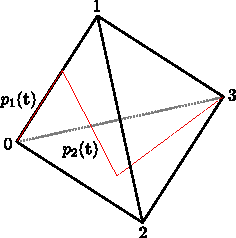
\includegraphics[scale=1]{aux/theta1.pdf}
	\caption{In red, the path $\theta_3(\bft) \in P(\gsimplex^3, v_0, v_3)$ associated to a $\bft \in \gcube^2$.}
	\label{f:theta1}
\end{figure}

A straightforward computation proves that the conditions in \cref{ss:adams maps} are satisfied by this collection.
A diagrammatical verification in low dimensions is provided in \cref{f:theta3}.

\begin{figure}[b]
	\centering
	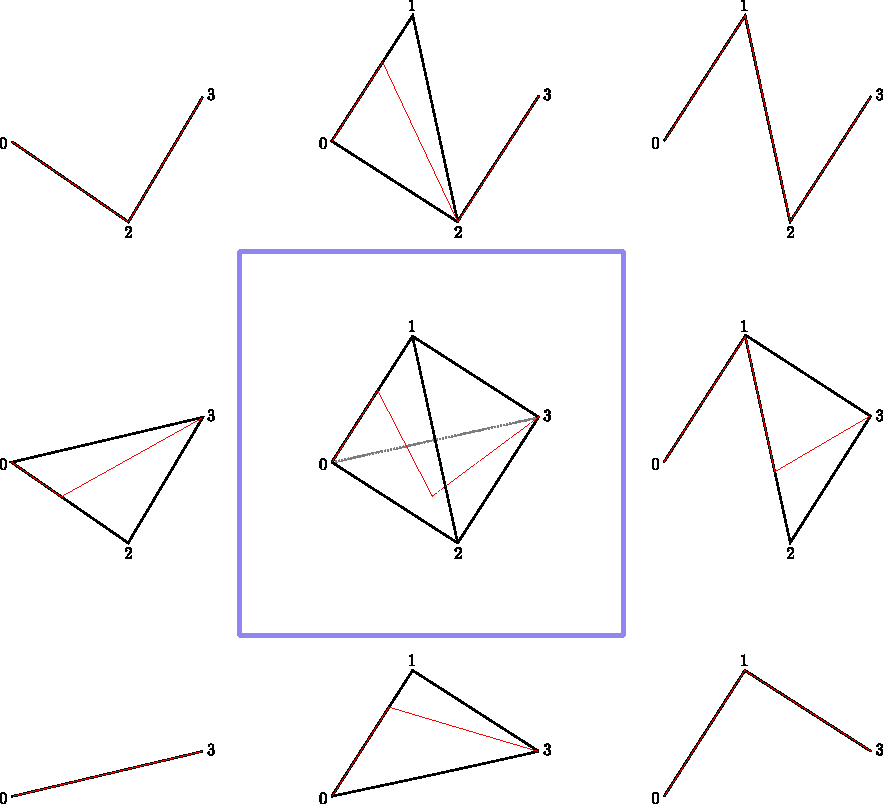
\includegraphics[scale=.5]{aux/theta3.pdf}
	\caption{The faces of the $2$-cube in blue, labeled by a red element in their corresponding family of paths.}
	\label{f:theta3}
\end{figure}

We can extend this collection $\{\theta_n \colon \gcube^{n-1} \to P(\gsimplex^n;v_0,v_n)\}$ to one of the form
\[
\set[\big]{\theta_{(n_1, \dots, n_k)} \colon \gcube^{n_1 + \dots + n_k-k} \to P(\gsimplex^{n_1} \vee \cdots \vee \gsimplex^{n_k})}
\]
where the \textit{topological necklace} $\gsimplex^{n_1} \vee \cdots \vee \gsimplex^{n_k}$ is obtained by identifying the last vertex of $\gsimplex^{n_i}$ with the first vertex of $\gsimplex^{n_{i+1}}$ for each $i = 1, \dots, k-1$ assuming each $n_i > 0$.
We do so by setting
\begin{multline*}
	\theta_{(n_1, \ldots, n_k)}(t_1, \ldots, t_{n_1+ \cdots + n_k-k}) \\ =
	\theta_{n_1}(t_1, \ldots, t_{n_1-1}) \cdot\ \dots\ \cdot \theta_{n_k}(t_{n_1+ \cdots n_{k-1}-k},\ldots,t_{n_1 + \cdots +n_k-k}).
\end{multline*}
Thus we can think of the topological necklace $\gsimplex^{n_1} \vee \cdots \vee \gsimplex^{n_k}$ as a space parameterizing a $(n_1+ \cdots + n_k-k)$-dimensional family of paths between the first and last vertices.
Please consult \cref{f:theta2} for an example illustrating this construction.

\begin{figure}
	\centering
	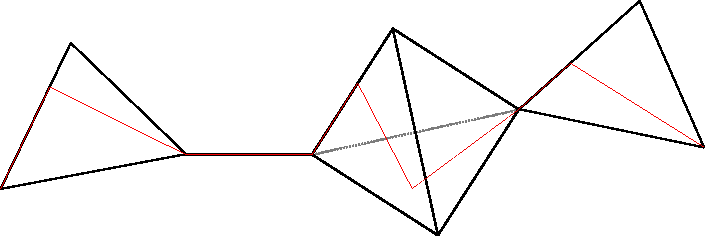
\includegraphics[scale=1]{aux/theta2.pdf}
	\caption{In red, the path $\theta_{(2,1,3,2)}(\bft)$ in $P(\gsimplex^2 \vee \gsimplex^1 \vee \gsimplex^3 \vee \gsimplex^2)$ associated to an element $\bft$ in $\gcube^{4}$.}
	\label{f:theta2}
\end{figure}

\subsection{Necklaces}

We now present a categorical viewpoint on the necklaces encountered in the previous subsection and their intimate relationship with Adams' cobar construction.
For any pointed space $(\fX,x)$, the underlying graded $\k$-module of $\cobar \sSchainsA(\fX,x)$ can be described as the graded $\k$-module freely generated by finite ordered sequences
\[
T = (\sigma_1, \dots, \sigma_k)
\]
of simplices $\sigma_i \in \sSing(\fX,x)$, with degree $\bars{T} = \bars{\sigma_1}+\dots+\bars{\sigma_k} - k$, modulo the sub $\k$-module generated by those sequences with at least one degenerate simplex.
The differential of $\cobar \sSchainsA(\fX,x)$ on a generator $T$ of degree $n$ is given by a signed sum of all generators $T'$ of degree $n-1$ that, in certain sense, fit inside $T$.
Furthermore, the monoid structure of $\cobar \sSchainsA(\fX,x)$ is induced by simply concatenating these ordered sequences of simplices.
This perspective suggests that $\cobar \sSchainsA(\fX,x)$ may be obtained by applying a normalized chains functor to certain cellular monoid, naturally associated to $(\fX,x)$, with cells labeled by finite ordered sequences of simplices in $\sSing(\fX,x)$.
A geometric construction reflecting this idea was described in \cite{baues1980geometry}.
We instead take a categorical approach and make this discussion precise through the framework of \textit{necklaces} and \textit{necklical sets} as we now discuss.

Consider the subcategory $\simplex_{*,*}$ of the simplex category $\simplex$ with the same objects and morphisms given by functors $f \colon [n] \to [m]$ satisfying $f(0) = 0$ and $f(n) = m$.
It is a strict monoidal category when equipped with the monoidal structure $[n] \ot [m] = [n+m]$, thought of as identifying the elements $n \in [n]$ and $0 \in [m]$, and unit given by $[0]$.
Heuristically, we may think of $\simplex_{*,*}$ as a category of models for cells parameterizing families of paths with fixed endpoints inside a simplex.

The \textit{necklace category} $\Nec$ is obtained from $\simplex_{*,*}$ as follows.
Thinking of $\simplex_{*,*}$ as a monoid in $\Cat$, we first apply the bar construction to it and produce a simplicial object in $\Mon_{\Cat}$ which, after realization, defines the strict monoidal category $\Nec$.
We denote the monoidal structure by
\[
\vee \colon \Nec \times \Nec \to \Nec.
\]
We describe $(\Nec, \vee)$ in more explicit terms.
The objects of $\Nec$, called \textit{necklaces}, are freely generated by the objects of $\simplex_{*,*}$ through the monoidal structure $\vee$.
Namely, the set of objects of $\Nec$ is the set of monomials
\[
\big\{ [n_1] \vee \dots \vee[n_k] \mid n_i, k \in \N_{>0} \big\}
\]
together with $[0]$ serving as the monoidal unit.

The morphisms of $\Nec$ are generated through the monoidal structure by the following four types of morphisms for all $n \in\N_{>0}$
\begin{enumerate}
	\item $\partial^j \colon [n-1] \to [n]$ for $j = 1, \dots, n-1$,
	\item $\Delta_{[j], [n-j]} \colon [j] \vee [n-j] \to [n]$ for $j = 1, \dots, n-1$,
	\item $\xi^j \colon [n+1] \to [n]$ for $j = 0, \dots, n$ and $n>0$, and
	\item $\xi^0 \colon [1] \to [0]$.
\end{enumerate}
We may identify $\Nec$ with a full sub-category of the category of double pointed simplicial sets $\sSet_{*,*}$ as follows.
Consider the functor
\[
\mathcal{S} \colon \Nec \to \sSet_{*,*}
\]
induced by sending any necklace $T = [n_1] \vee \dots \vee[n_k]$ to the simplicial set
\[
\mathcal{S}(T) = \simplex^{n_1} \vee \dots \vee \simplex^{n_k},
\]
where the wedge symbol now means we identify the last vertex of $\simplex^{n_i}$ with the first vertex of $\simplex^{n_{i+1}}$ for $i = 1, \dots, k-1$ and the two base points are given by the first vertex of $\simplex^{n_1}$ and the last vertex of $\simplex^{n_k}$.
Then $\mathcal{S}$ is a fully faithful functor, so $\Nec$ may be identified with the full sub-category of $\sSet_{*,*}$ having as objects those double pointed simplicial sets of the form $\simplex^{n_1} \vee \dots \vee \simplex^{n_k}$.
The \textit{dimension} of a necklace $T = [n_1] \vee\dots\vee [n_k]$ is defined by $\dim(T) = n_1 + \dots + n_k-k$.
Note there is a canonical homeomorphism \[\gsimplex^{n_1} \vee \cdots \vee \gsimplex^{n_k} \cong | \simplex^{n_1} \vee \cdots \vee \simplex^{n_k}|.\]

The category of \textit{necklical sets} $\Fun(\Nec^{\op}, \Set)$ becomes a (non-symmetric) monoidal category with monoidal structure induced from $(\Nec, \vee)$.
We denote the monoidal category of necklical sets by $\nSet$.

\begin{remark*}
	The category of necklaces was introduced in \cite{dugger2011rigidification} to give an explicit description of the homotopy coherent nerve functor and its left adjoint.
\end{remark*}

\subsection{From necklaces to cubes}

In \cref{explicitchoice} we described an explicit way of decomposing a topological necklace $\gsimplex^{n_1} \vee \cdots \vee \gsimplex^{n_k}$ into a family of paths connecting the first and last vertices parameterized by an $(n_1 + \cdots + n_k-k)$-dimensional cube.
This construction satisfies conditions (1), (2), and (3) in \cref{ss:adams maps}.
In particular, conditions (2) and (3) may be interpreted as saying that each face in the codimension $1$ boundary of such a cube of paths is in one-to-one correspondence with codimension $1$ ``sub-necklaces" inside $\gsimplex^{n_1} \vee \cdots \vee \gsimplex^{n_k}$ connecting the first and last vertices.
Furthermore, sub-necklaces in $\gsimplex^{n_1} \vee \cdots \vee \gsimplex^{n_k}$ are in one-to-one correspondence with the poset \[\{ J \subseteq \{0,\ldots, n_1+ \cdots + n_k-k\} | 0,n_1+ \cdots +n_k-k \in J \}\]
ordered by inclusion, which has a canonical cubical structure.
We build upon this observation to describe a functorial relation between necklaces and cubes.
This will be used to explain how Adams' map is induced by a deeper categorical construction.

We begin by defining a monoidal functor
\[
\cP \colon \Nec \to \cube
\]
as follows.
First define $\cP[0] = 2^0$.
On any other necklace $T \in \Nec$, define $\cP(T) = 2^{\dim(T)}$.
In order to define $\cP$ on morphisms, it is sufficient to consider the following cases.
\begin{enumerate}
	\item For any coface map $\partial^j \colon [n] \to [n+1]$ such that $0< j<{n+1}$, define $\cP(\partial^j) \colon 2^{n-1}\to 2^{n}$ to be the cubical coface functor $\cP(f)= \delta_0^{j}$.

	\item For any $\Delta_{[j], [n+1-j]} \colon [j] \vee [n+1-j] \to [n+1]$ such that $0<j<n+1$, define
	\[
	\cP(\Delta_{[j], [n+1-j]}) \colon 2^{n-1}\to 2^{n}
	\]
	to be the cubical coface functor $\cP(f)=\delta_1^{j}$.

	\item We now consider codegeneracy maps of the form $\xi^j \colon [n+1] \to [n]$ for $n>0$.
	If $j=0$ or $j=n$, define $\cP(f) \colon 2^n \to 2^{n-1}$ to be the cubical codegeneracy functor $\cP(s^j)= \varepsilon^{j}$.
	If $0<j<n$, define $\cP(s^j) \colon 2^n \to 2^{n-1}$ to be the cubical coconnection functor $\gamma^{j}$.

	\item For $\xi^0 \colon [1] \to [0]$ define $\cP(\xi^0) \colon 2^0 \to 2^0$ to be the identity functor.
\end{enumerate}

\begin{remark*}
	The functor $\cP$ is neither faithful or full.
	However, for any necklace $T' \in \Nec$ with $\dim(T')=n+1$ and any cubical coface functor $\delta_{\epsilon}^j \colon 2^n \to 2^{n+1}$ for $0 \leq j \leq n+1$, there exists an map $f \colon T \hookrightarrow T'$, where $T \in \Nec$ with $\dim(T)=n$ such that $\mathcal{S}(f) \colon \mathcal{S}(T) \hookrightarrow \mathcal{S}(T')$ is an injective morphism in $\Nec$ and $\cP(f) = \delta_{\epsilon}^j$.
\end{remark*}

The functor $\cP \colon \Nec \to \cube$ induces an adjunction between $\cSet$ and $\nSet$ with right and left adjoint functors given respectively by
\[
\cP^\ast \colon \cSet \to \nSet,
\qquad \text{and} \qquad
\cP_{!} \colon \nSet \to \cSet.
\]
Explicitly, for a cubical set $Y \colon \cube^\op \to \Set$,
\[
\cP^\ast(Y)= Y \circ \cP^\op,
\]
and for a necklical set $K \colon \Nec^\op \to \Set$,
\[
\cP_{!}(K) \ =
\colim_{\mathcal{Y}(T) \to K} \cP(T) \ \cong
\colim_{\mathcal{Y}(T) \to K} \cube^{\dim(T)}.
\]
Since $\cP$ is a monoidal, the functor $\cP_{!} \colon \nSet \to \cSet$ is monoidal as well.

\subsection{Cubical cobar construction}\label{ss:cubical cobar}

Using the framework of necklical sets, we may reinterpret Baues' geometric cobar construction \cite{baues1980geometry} as a functor
\[
\ncobar \colon \sSet^0 \to \Mon_{\nSet},
\]
which we now define.

For any reduced simplicial set $X$, we define a necklical set $\ncobar(X) \colon \Nec^\op \to \Set$ having as necklical cells all necklaces inside $X$; namely
\[
\ncobar(X) \, = \! \colim_{\mathcal{S}(T) \to X} \mathcal{Y}(T).
\]
The monoidal structure $\vee \colon \Nec \times \Nec \to \Nec$ given by concatenation of necklaces induces a natural product
\[
\ncobar(X) \ot \ncobar(X) \to \ncobar(X)
\]
making $\ncobar(X)$ into a monoid in $\nSet$.

We may now define the \textit{cubical cobar construction}
\[
\ccobar \colon \sSet^0 \to \Mon_{\cSet}
\]
as the composition
\[
\ccobar = \cP_! \, \circ \ncobar.
\]
Since $\cP_!$ is monoidal, $\ccobar(X)$ is a monoid in $\cSet$.

\begin{remark}
	This reinterpretation of Baues' construction in terms of cubical sets was also studied in \cite{rivera2018cubical}.
	In this reference, it is also proven that the composition of functor $\mathcal{T} \circ \ccobar$, where $\mathcal{T} \colon \Mon_{\cSet} \to \Mon_{\sSet}$ is the triangulation functor, coincides with the left adjoint of the homotopy coherent nerve functor restricted to $\sSet^0.$
\end{remark}

\subsection{Relation to the cobar construction}

We now relate the cubical cobar functor $\ccobar \colon \sSet^0 \to \Mon_{\cSet}$ to the cobar construction $\cobar \colon \coAlg^\ast \to \Mon_{\Ch}$ (\cref{ss:cobar construction}).

\begin{theorem}\label{t:ccobar and cobar}
	There is a natural isomorphisms of functors
	\[
	\cchains \ccobar \cong \cobar \schainsA \colon \sSet^0 \to \Mon_{\Ch}.
	\]
\end{theorem}

\begin{proof}
	Denote by $\iota_n \in (\cube^n)_n$ the top dimensional non-degenerate element of the standard $n$-cube $\cube^n$.
	Note that for a reduced simplicial set $X$, we may represent any non-degenerate $n$-cube $\alpha \in (\cP_!(\ncobar(X)))_n$ as a pair $\alpha = [\sigma \colon \mathcal{Y}(T) \to X, \iota_n]$ for some $T = [n_1] \vee \dots \vee [n_k] \in \Nec$ with $\dim(T) = n_1 + \dots + n_k - k = n$.

	To define a monoidal chain map
	\[
	\varphi_X \colon \cchains(\cP_!(\ncobar(X))) \xra{\cong} \cobar \schainsA(X)
	\]
	it suffices to define it on any generator of the form $\alpha=[\sigma \colon \simplex^{n+1} \to X, \iota_{n}]$, i.e., when $T$ is of the form $T = [n+1]$, for some $n \geq 0$.
	If $n = 0$ let $\varphi_X(\alpha)= [\overline{\sigma}] + 1_\k$, where $[\overline{\sigma}] \in \s{-1} \overline{ \schains(X)} \subset \cobar \schainsA(X)$ denotes the (length $1$) generator in the cobar construction of $\schains(X)$ determined by $\sigma \in X_{n+1}$ and $1_\k$ denotes the unit of the underlying ring $\k$.
	If $n > 0$, we let $\varphi_X(\alpha)=[\overline{\sigma}]$.
	A straightforward computation yields that this gives rise to a well defined isomorphism of algebras, which is compatible with the differentials, and natural with respect to maps of simplicial sets.
\end{proof}

A similar result to \cref{t:ccobar and cobar} was observed in the case of $1$-reduced simplicial sets in \cite[Section~3.5]{berger1995loops}.

\subsection{Factorization of Adams's map}\label{ss:factorization of adams}

Adams's comparison map can be factored as a composition
\begin{equation}\label{e:factorization of adams}
	\theta_\fX \colon \cobar \sSchainsA(\fX,x) \xrightarrow{\cong}
	\cchains \ccobar(\sSing(\fX,x)) \xrightarrow{\cchains(\Theta)}
	\cSchains(\loops_x \fX).
\end{equation}
The first map is the monoidal isomorphism induced by \cref{t:ccobar and cobar}.
The second map is given by applying chains $\cchains \colon \Mon_{\cSet} \to \Mon_{\Ch}$ to the map of monoidal cubical sets
\[
\Theta \colon \ccobar(\sSing(\fX,x)) \to \cSing(\loops_x \fX)
\]
determined through the monoid structure by sending an $n$-simplex $(\sigma \colon \gsimplex^n \to \fX)$ to the singular $(n-1)$-cube
\[
P(\sigma) \circ \theta_n \colon \gcube^{n-1} \to \loops_x \fX,
\]
where the maps $\theta_n \colon \gcube^{n-1} \to P(\gsimplex^n;0,n)$ are discussed in \cref{ss:adams maps}.

\subsection{A monoidal coalgebra structure on the cobar construction}

We follow \cite{baues1998hopf} to construct a coalgebra structure on $\cobar \sSchainsA(\fX,x)$, compatible with both the differential and monoid structure, such that Adams's map becomes a map of monoids in the category of coalgebras.

Recall the Serre coalgebra lift $\cchainsA \colon \cSet \to \coAlg$ of $\cchains \colon \cSet \to \Ch$, the unique monoidal functor defined by the coalgebra structure on $\chains(\cube^1)$.
Since $\cchainsA$ is monoidal and $\ccobar(\sSing(\fX,x))$ is a monoid, $\cchainsA(\ccobar(\sSing(\fX,x)))$ is a monoid in $\coAlg$.
Similarly, the lift $\cchainsA$ equips $\cSing(\loops_x \fX)$ with a natural monoidal coalgebra structure as well.
Consequently, the isomorphism in (\ref{e:factorization of adams}) endows $\cobar \sSchainsA(\fX,x)$ with a natural monoidal coalgebra structure making $\theta_\fX$ into natural map of monoidal coalgebras.
	% !TEX root = ../cobar1.tex

\section{Monoidal \pdfEinfty-structures}

\todo{@anibal: Write mini-intro for s:monoidal e-infty}
talking points

that is a cofibrant resolution of the terminal operad -- which controls cocommutative and coassociative coalgebras.

\subsection{$\cM$-bialgebras}

\begin{definition*}
	An $\cM$-bialgebra is a coalgebra $(C, \Delta, \aug)$ together with a degree~1 product satisfying for any $a,b \in C$ that:
	\begin{align}
		\label{eq:M-bialg def 1}
		\aug(a \ast b) =\ & 0, \\
		\label{eq:M-bialg def 2}
		\bd (a \ast b) =\ & \bd a \ast b - (-1)^{a} a \ast \bd b + \aug(a) b - (-1)^{a} a \aug(b).
	\end{align}
\end{definition*}

\begin{remark*}
	\cref{eq:M-bialg def 2} states that the product, regarded as an element in the chain complex $\Hom(C \ot C, C)$, has boundary equal to $\aug \ot\, \id - \id \ot \aug$.
	% PROOF
	%\begin{align*}
	%	(\bd \ast)(x \ot y) =\ & (\aug \ot\, \id - \id \ot \aug)(x \ot y), \\
	%	(\bd \circ \ast + \ast \circ (\bd \ot\, \id + \id \ot \bd))(x \ot y) =\ & \aug(x) \ot\, y - x \ot \aug(y), \\
	%	(-1)^x \bd (x \ast y) + (-1)^{x-1} \bd x \ast y + x \ot \bd y =\ & \aug(x) \ot\, y - x \ot \aug(y), \\
	%	\bd (x \ast y) =\ & \bd x \ast y + (-1)^{x+1} x \ast \bd y + \aug(x) y + (-1)^{x+1} x \aug(y).
	%\end{align*}
\end{remark*}

\begin{proposition*}[\cite{medina2020prop1}]
	Let $(C, \Delta, \aug, \ast)$ be an $\cM$-bialgebra.
	The collection of all maps $\set{C \to C^{\ot r}}_{r \in \N}$ generated by $\Delta$, $\aug$ and $\ast$ makes $C$ into an $E_\infty$-coalgebra.
	More specifically, into a coalgebra over the model $\UM$ of the $E_\infty$-operad.
\end{proposition*}

\begin{remark*}
	The operad $\UM$ is obtained from a prop $\M$ by restricting its structure to biarities $(1,r)$ for $r \in \N$.
\end{remark*}

\begin{example}[\cite{medina2020prop1}]\label{ex:simplicial e-infty}
	The Alexander--Whitney coalgebra $\chains(\simplex^n)$ can be made into a natural $\cM$-bialgebra considering an algebraic version of the \textit{join product} defined by
	\begin{equation*}
		\left[v_0, \dots, v_p \right] \ast \left[v_{p+1}, \dots, v_q\right] =
		\begin{cases} (-1)^{p} \sign(\pi) \left[v_{\pi(0)}, \dots, v_{\pi(q)}\right] &
			\text{ if } v_i \neq v_j \text{ for } i \neq j, \\
			\hfil 0 & \text{ if not},
		\end{cases}
	\end{equation*}
	where $\pi$ is the permutation that orders the vertices.
	A Kan extension of the associated $\UM$-coalgebra defines a lift of the Alexander--Whitney coalgebra structure into the category of $E_\infty$-coalgebras defined by $\UM$.
	Diagrammatically, we have
	\begin{equation*}
		\begin{tikzcd}[column sep=normal, row sep=small]
			& \coAlg_{\UM} \arrow[d] \\
			\sSet \arrow[r]
			\arrow[ur,out=60, in=180, dashed, "\schainsUM"]
			\arrow[r, "\schainsA"]
			& \coAlg,
		\end{tikzcd}
	\end{equation*}
	where the vertical arrow is the obvious forgetful functor.
\end{example}

\begin{example}[\cite{medina2022cube_einfty}]\label{ex:cubical e-infty}
	The Serre coalgebra coalgebra $\chains(\cube^n)$ can be made into a natural $\cM$-bialgebra considering a product defined using the following notation.
	For a basis element $x = x_1 \ot \dotsb \ot x_n$ of $\chains(\cube^n)$ and an integer $\ell \in \set{1,\dots,n}$ we write
	\begin{align*}
		x_{<\ell} & = x_1 \ot \dotsb \ot x_{\ell-1}, \\
		x_{>\ell} & = x_{\ell+1} \ot \dotsb \ot x_n,
	\end{align*}
	with the convention $x_{<1} = x_{>n} = 1 \in \Z$.
	Then, for two such basis elements $x$ and $x'$ we set
	\begin{multline*}
		(x_1 \ot \dotsb \ot x_n) \ast (x'_1 \ot \dotsb \ot x'_n)
		=
		(-1)^{|x|} \sum_{i=1}^n x_{<i}\, \epsilon(x'_{<i}) \ot x_i \ast x'_i \ot \epsilon(x_{>i}) \, x'_{>i},
	\end{multline*}
	where the only non-zero values of $x_i \ast x'_i$ are
	\[
	[0] \ast [1] = [0, 1], \qquad [1] \ast [0] = -[0, 1].
	\]
	As in the simplicial case, a Kan extension of the $\UM$-coalgebra structure on $\chains(\cube^n)$ defines a lift of the Serre coalgebra structure into the category of $E_\infty$-coalgebras defined by $\UM$.
	Diagrammatically, that is
	\begin{equation}\label{eq:lift to e-infty cubical}
		\begin{tikzcd}[column sep=normal, row sep=small]
			& \coAlg_{\UM} \arrow[d] \\
			\cSet \arrow[r]
			\arrow[ur,out=60, in=180, dashed, "\cchainsUM"]
			\arrow[r, "\cchainsA"]
			& \coAlg.
		\end{tikzcd}
	\end{equation}
\end{example}

\subsection{Tensor product of $\cM$-bialgebras}

In this section we describe an extension of the tensor product of coalgebras to $\cM$-bialgebras, and observe that the lift of the Serre coalgebra structure to $\UM$-coalgebras is a monoidal functor.

\begin{lemma}\label{l:monoidal M-bialg}
	Let $C$ and $C'$ be $\M$-bialgebras.
	The coalgebra $C \ot C'$ is a natural $\M$-bialgebra with
	\begin{equation}\label{eq:monoidal_product}
		(a \ot b) \ast (c \ot d) =
		a \aug(c) \ot (b \ast d) + (a \ast c) \ot \aug(b) d,
	\end{equation}
	for any $a,c \in C$ and $b,d \in C'$.
\end{lemma}

The proof of this lemma is a straightforward computation which for completeness is presented in \cref{s:appendix}.

\begin{remark}
	The prop $\cM$ controlling $\cM$-bialgebras is obtained by applying the functor of chains to a cellular prop whose cells are cubical \cite{medina2021prop2}.
	The product is represented by a cell isomorphic to the interval $[01]$, with $[1]$ corresponding to $\aug \ot \, \id$ and $[0]$ to $\id \ot \aug$.
	\cref{eq:monoidal_product} comes from the diagonal $[01] \mapsto [0] \ot [01] + [01] \ot [1]$.
	In fact, if so inclined, one can observe that both $\cM$ and $\UM$ are defined over coalgebras and not just chain complexes.
\end{remark}

\anibal{Proof for this:}

It can be inspected that using this theorem on $\chains(\cube^n) \cong \chains(\cube^1)^{\ot n}$ one recovers the $\cM$-bialgebra described in \cref{ex:cubical e-infty}.
Since for any two cubical sets $X$ and $X'$ we have $\chains(X \times X') \cong \chains(X) \ot \chains(X')$ the above lemma implies the following statement.

\begin{theorem}\label{t:cubical e-infty chains are monoidal}
	The functor $\cchainsUM$ extending the Serre coalgebra structure to an $E_\infty$-coalgebra structure is monoidal.
\end{theorem}

\subsection{A monoidal \pdfEinfty-coalgebra structure on the cobar construction}\label{ss:e-infty on cobar}

%The original cobar construction of Adams produces a monoid in $\Ch$ from a connected coalgebra. Baues enriched this construction to produce a monoid in $\coAlg$.
%He did this by using a version of the isomorphism $\cchains \ccobar \cong \cobar \schainsA$ of \cref{t:ccobar and cobar} and the Serre coalgebra on cubical chains.
%Since $\ccobar$ produces monoids in $\cSet$ and $\cchainsA$ is monoidal, the functor $\cchainsA \ccobar$ produces bialgebras, as claimed.

We now use the natural equivalence of functors $\cchains \ccobar \cong \cobar \schainsA$ proven in \cref{t:ccobar and cobar} to transfer structure.

After \cite{medina2022cube_einfty}, we know that cubical chains can be enriched with an $E_\infty$-coalgebra structure extending the Serre coalgebra (\cref{ss:e-infty on cubical}).
This $\UM$-structure can be transferred via $\cchains \ccobar \cong \cobar \schainsA$ to provide the cobar construction with and $E_\infty$-structure extending Baues coalgebra structure.
Furthermore, thanks to \cref{t:cubical e-infty chains are monoidal}, we know that $\cchainsUM$ is monoidal and therefore, $\cchains \ccobar$ produces monoids in $\coAlg_{\UM}$, i.e., $E_\infty$-bialgebras.
This discussion proves the first half of \cref{t:1st main thm in the intro}, which we collect in the following.

\begin{lemma}\label{l:lift of cobar to e-infty}
	The functor $\cchainsUM$ is monoidal and fits in the following diagram commuting up to a natural isomorphism:
	\[
	\begin{tikzcd}
		& \Mon_{\coAlg_\UM} \arrow[d] \\
		\Mon_{\cSet} \arrow[ru, "\cchainsUM", out=70, in=180] \arrow[r, "\cchainsA"]
		& \Mon_{\coAlg} \arrow[d] \\
		\sSet^0 \arrow[r, "\cobar \schainsA"] \arrow[u, "\ccobar"]
		& \Mon_{\Ch}.
	\end{tikzcd}
	\]
\end{lemma}

\subsection{Steenrod operations}

Throughout this subsection let us consider $\k$ to be the finite field $\Fp$ and $X$ a reduced simplicial set.

Since $\cobar \schainsA(X)$ is isomorphic to the chains on a cubical set (\cref{t:ccobar and cobar}), its mod $p$ homology is a priori equipped with a right action of the Steenrod algebra \cite{steenrod1962cohomology, milnor1958steenrod}.
As an application of the explicit construction of a natural $\UM$-coalgebra structure on $\cobar \schainsA(X)$, we can describe the chain level this action using the constructions of \cite{medina2021may_st}.
More explicitly, let $\Cp$ be the cyclic group of order $p$ and
\[
\begin{tikzcd} [column sep = .5cm]
	\cW(p) = \Fp[\Cp]\{e_0\} & \arrow[l, "\,T"'] \Fp[\Cp]\{e_1\} & \arrow[l, "\,N"'] \Fp[\Cp]\{e_2\} & \arrow[l, "\,T"'] \dotsb
\end{tikzcd}
\]
be the minimal free resolution of $\Fp$ as an $\Fp[\Cp]$-module.
Consider the $\Cp$-equivari-ant quasi-isomorphism $\psi_\UM \colon \cW(p) \to \UM(p)$ constructed in \cite{medina2021may_st}, and denote by $\psi^{\cobar}$ its composition with the morphism $\UM \to \End^{\cobar \schainsA(X)}$ defining our $E_\infty$-coalgebra structure on $\cobar \schainsA(X)$.

If $p$ is the even prime, the Steenrod square $P_s$ is represented by the map sending a representative $\mu$ of a class in the $k^\th$ homology of $\cobar \schainsA(X)$ to the following element in its double linear dual:
\[
\mu \mapsto
\Big( \alpha \mapsto (\alpha \ot \alpha) \big( \psi^{\cobar}(e_{k+2s})(\mu) \big) \Big).
\]
Similarly, if $p$ is an odd prime, the action of the Steenrod operations $\beta^\varepsilon P_{s}$ where $\varepsilon = 0,1$ are represented by
\[
\mu \mapsto
\Big( \alpha \mapsto \alpha^{\ot p} \big( (-1)^p \, \nu(q) \, \psi^{\cobar}(e_{(2s-q)(p-1)-\varepsilon})(\mu) \big) \Big)
\]
where
\[
q = -k -2s(p-1) + \varepsilon, \qquad
\nu(q) = (-1)^{q(q-1)m/2}(m!)^q, \qquad
m = (p-1)/2.
\]

The map $\psi^{\cobar}$, being a special case of the map $\psi^\cube$ defined in \cite{medina2021may_st}, can be described effectively, and it has been implemented in the specialized computer algebra system \texttt{ComCH} \cite{medina2021comch}.
In similar effective manner, explicit Cartan and Adem coboundaries \cite{medina2020cartan, medina2021adem} can be described, in the $p = 2$ case, for cochain level Steenrod squares of the cobar construction of $\schains(X)$.


\subsection{Adams's map as a monoidal \pdfEinfty-coalgebra quasi-isomorphism}

Adams' comparison map
\[
\theta_Z \colon \cobar \sSchainsA(Z,z) \to \cSchains(\loops_z Z)
\]
was originally identified to be a morphism of monoids in $\Ch$ which, if applied to simply-connected spaces, induces a homology isomorphism.
Baues showed that $\theta_Z$ is in fact a morphism of monoids in $\coAlg$, i.e., of bialgebras.
Whereas, using that $\sSing(Z,z)$ is a fibrant reduced simplicial set, the second named author and M. Zeinalian \cite{rivera2018cubical} showed that for a possibly non-simply connected pointed space $(Z,y)$ the algebras $\cobar \sSchainsA(Z,z)$ and $\cSchains(\loops_zZ)$ are quasi-isomorphic.
Later on, the second named author and S. Saneblidze
\cite{rivera2019path} showed that $\Theta \colon \ccobar(\sSing(Z,z)) \to \cSing(\loops_z Z)$ is a weak homotopy equivalence of monoids in $\cSet$.

We now show that $\theta_Z$ is in fact a quasi-isomorphism of $E_{\infty}$-bialgebras.
Considering the factorization \eqref{e:factorization of adams} of Adams' comparison map.
The isomorphism is by construction one of $\UM$-bialgebras, whereas the second map, induced from a weak-equivalence of monoids in $\cSet$, is also a morphism of $\UM$-bialgebras
since $\cchainsUM$ is monoidal (\cref{t:cubical e-infty chains are monoidal}).
We summarize this discussion, which constitutes the second half of \cref{t:1st main thm in the intro}, in the following.

\begin{lemma}\label{l:adams comparison is an e-infty bialgebra map}
	Adams' comparison map $\theta_Z \colon \cobar \sSchainsA(Z,z) \to \cSchains(\loops_z Z)$ is a quasi-isomorphism of $E_{\infty}$-bialgebras or, more specifically, of monoids in $\coAlg_\UM$ for any pointed space $(Z,z)$.
\end{lemma}
	\sloppy
    \printbibliography
%    %Recall that for any pointed topological space $(\fZ,z)$ there is a naturally associated topological monoid $\loops_z \fZ$ -- its \textit{based loop space} -- whose points are pairs $(\gamma, r)$ where $r \in \R_{\geq 0}$ and $\gamma \colon [0,r] \to \fZ$ is a continuous map with $\gamma(0) = z = \gamma(r)$.
%We consider $\loops_z \fZ$  equipped with the compact-open topology and the continuous multiplication defined by \textit{concatenation} of loops.
\todo{@manuel: this is important because of ...}
%whose identity element is the \textit{constant loop} $(c_r,0)$.
%For any loop $\gamma \colon [0,r] \to \fZ $ its concatenation with the loop $\overline{\gamma} \colon [0,r] \to \fZ$ which runs $\gamma$ in the opposite direction, namely $\overline{\gamma}(t) = \gamma(r-t)$, is homotopic to the constant loop.
%Consequently, we may say that $\loops_z \fZ$ has inverses \textit{up to homotopy}, and we have that the set of path components $\pi_0(\loops_z \fZ)$ has an induced group structure naturally isomorphic to the fundamental group $\pi_1(\fZ,z)$.
%Furthermore, $\loops_z \fZ$ is weak homotopy equivalent to a topological group where the group identities hold strictly \cite{milnor1956bundles}, \cite{berger1995loops}.
%The pointed space $(\fZ,z)$ may then be recovered, up to weak homotopy equivalence, from the weak homotopy type of the topological monoid $\loops_z \fZ$ through the \textit{classifying space}, or \textit{delooping}, construction.

%One of the principal goals of algebraic topology is to encode the theory of topological spaces up to some specified notion of equivalence in terms of combinatorial or algebraic objects, allowing for the effective analysis of topological properties.
%We will focus on spaces up to weak homotopy equivalence, where a first example of an algebraization procedure is provided by the functor of simplicial or cubical singular chains
%\[
%\Schains \colon \Top \to \Ch,
%\]
%which associates a chain complex over a fixed commutative ring to any topological space.

%In this work we are interested in approximating the homotopy type of this topological monoid $\loops_z \fZ$ by monoids in chain complexes with additional structure.

%, a purely algebraic functor
%\[
%\cobar \colon \coAlg^\ast \to \Mon_{\Ch},
%\]

%Diagrammatically, this can be represented as lifts of the form
%\begin{equation}
%	\begin{tikzcd}[column sep=normal, row sep=small]
	%		& \coAlg_{E_\infty} \arrow[d] \\
	%		& \coAlg \arrow[d] \\
	%		\Top \arrow[uur, "\Schains_{E_\infty}", out=90, in=180] \arrow[r, "\Schains"]
	%		\arrow[ur, "\SchainsA", out=60, in=180, near end]
	%		\arrow[r, "\Schains"]
	%		& \Ch.
	%	\end{tikzcd}
%\end{equation}
%The study of $E_\infty$-structures has a long history, where (co)homology operations \cite{steenrod1962cohomology, may1970general}, the recognition of infinite loop spaces \cite{boardman1973homotopy, may1972geometry}, and the complete algebraic representation of the $p$-adic homotopy category \cite{mandell2001padic} are key milestones.

%For based loop spaces we will consider two algebraic models which we now describe for a pointed space $(Z, z)$.
%The first is given by the cubical singular chains $\cSchains(\loops_z Z)$ which, as we recall below, is a monoid in $\Ch$.
%The second, introduced by F.~Adams in \cite{adams1956cobar}, is defined by applying his \textit{cobar construction}
%\[
%\cobar \colon \coAlg^\ast \to \Mon_{\Ch},
%\]
%a functor from coaugemented (dg) coassociative coalgebras to monoids in $\Ch$, to the coalgebra of pointed simplicial singular chains $\sSchainsA(\fZ, z)$.
%In the same reference, Adams constructed a comparison map between these models, a natural chain map of monoids in $\Ch$
%\begin{equation} \label{e:adams map}
%	\theta_Z \colon \cobar \sSchainsA(\fZ, z) \to \cSchains(\loops_z Z),
%\end{equation}
%which he proved to be a quasi-isomorphism if $Z$ is simply connected, a result extended to path-connected spaces in \cite{rivera2018cubical} by considering finer homotopical algebra, and in \cite{hess2010cobar} by a localization procedure.
%
%In this article we enhance both of these models by explicitly constructing an $E_\infty$-bialgebra structure on them, i.e., an $E_\infty$-coalgebra structure compatible with its monoid structure, and show that Adams' comparison map is a quasi-isomorphism of $E_\infty$-bialgebras.

%Our starting point is groundbreaking work by H.~Baues proving similar statements to ours.
%that allowed him to accomplish analogous statements using monoids in coalgebras instead of in $E_\infty$-coalgebras.
%His insights are best explained in terms of \textit{cubical sets} (with connections).
%, i.e., objects in the category $\cSet$ of presheaves over the strict monoidal category generated by the diagram
%\[
%\begin{tikzcd}
%	1 \arrow[r, out=45, in=135, "\delta^0"] \arrow[r, out=-45, in=-135, "\delta^1"'] & 2 \arrow[l, "\sigma"'] &[-10pt] \arrow[l, "\gamma"'] 2 \times 2
%\end{tikzcd}
%\]
%restricted by certain relations \cite{brown1981cubes}.
%With the Day convolution monoidal structure on $\cSet$, the cubical singular complex functor $\cSing \colon \cSet \to \Top$ and the functor of (normalized) chains $\cchains \colon \cSet \to \Ch$ are both monoidal, which explains the monoid structure on
%\[
%\cSchains(\loops_z Z) \defeq \cchains \cSing(\loops_z Z).
%\]
%Furthermore, cubical chains are equipped with a natural coalgebra structure coming from Serre's chain approximation to the diagonal.
%This structure provides a lift of $\cchains$ to the category of coalgebras via a monoidal functor
%\[
%\cchainsA \colon \cSet \to \coAlg.
%\]
%In particular, this construction makes $\cSchainsA(\loops_z Z) = \cchainsA\cSing(\loops_z Z)$ into a bialgebra, i.e., a monoid in $\coAlg$.



%Furthermore, Adams' comparison map
%\[
%\theta_Z \colon \cobar \sSchainsA(\fZ, z) \to \cSchains(\loops_z Z)
%\]
%is a quasi-isomorphism of $E_{\infty}$-bialgebras for any pointed space $(\fZ, z)$.
%
%Regarding Adams' comparison map, Baues showed that it factors as a composition
%\begin{equation} \label{e:baues factorization of adams map}
%	\begin{tikzcd}[column sep = small]
	%		\theta_Z \colon \cobar \sSchainsA(\fZ, z) \arrow[r] &
	%		\cchainsA\big(\!\ccobar \sSing(\fZ, z)\big) \arrow[r] &
	%		\cSchainsA(\loops_z Z),
	%	\end{tikzcd}
%\end{equation}
%where the first chain map is an isomorphism and the second is induced from an inclusion
%\[
%\ccobar \sSing(\fZ, z) \to \cSing(\loops_z Z)
%\]
%of monoids in $\cSet$, which is a weak equivalence following \cite{rivera2019path}.
%
%The first map in \eqref{e:baues factorization of adams map} is defined for a general reduced simplicial set $X$ and it is always an isomorphism.
%This permitted Baues to transfer the Serre coalgebra structure on $\cchainsA \ccobar(X)$ to $\cobar \schainsA(X)$ and show it compatible with the monoid structure.
%In other words, Baues' lifted Adams' cobar construction $\cobar \schainsA$ so that it fits in the following diagram commuting up to a natural isomorphism:
%\[
%\begin{tikzcd}
%	\Mon_{\cSet} \arrow[r, "\cchainsA \ "] & \Mon_{\coAlg} \arrow[d] \\
%	\sSet^0 \arrow[r, "\cobar \schainsA"] \arrow[u, "\ccobar"] & \Mon_{\Ch}.
%\end{tikzcd}
%\]
%
%The first result presented in this article is the construction of a lift of $\cchainsA \ccobar \colon \sSet^0 \to \Mon_{\coAlg}$ to the category of monoids in $\coAlg_\UM$, where $\coAlg_\UM$ is the category of coalgebras over the operad $\UM$ introduced via a finitely presented prop in \cite{medina2020prop1}.
%This is a model of the $E_\infty$-operad that explicitly acts on both simplicial and cubical chains.
%For this lift to be meaningful, we first need to define a monoidal structure on $\coAlg_\UM$.
%We do so by introducing a Hopf structure on $\UM$, that is to say, by making it into an operad over $\coAlg$, a structure that has other potential applications \cite{livernet2008hopf}.
%Once we have shown that $\coAlg_\UM$ is a monoidal category, we prove the main technical result of this work; that the lift
%\[
%\cchainsUM \colon \cSet \to \coAlg_\UM
%\]
%of $\cchainsA$ defined in \cite{medina2022cube_einfty} is monoidal.
%
%This has consequences for both algebraic models for the based loop space considered so far.
%Let $(\fZ, z)$ be a pointed space and $X$ a reduced simplicial set, for example $X = \sSing(\fZ, z)$.
%Since $\cSing(\loops_z Z)$ and $\ccobar X$ are monoids in $\cSet$ we have that both $\cSchainsUM(\loops_z Z)$ and $\cchainsUM \ccobar(X) \cong \cobar \schainsA(X)$ are monoids in $\coAlg_\UM$.
%Furthermore, if $X = \sSing(\fZ, z)$, Adams' comparison map $\theta_Z$ preserves this additional structure.
%We condense this discussion in our first main result.
%
%\begin{theorem*}
%	The functor $\cchainsUM$ is monoidal and its associated functor on monoids fits in the following diagram commuting up to a natural isomorphism:
%	\[
%	\begin{tikzcd} [row sep=small]
	%		& \Mon_{\coAlg_\UM} \arrow[d] \\
	%		\Mon_{\cSet} \arrow[ru, "\cchainsUM", out=70, in=180, near start] \arrow[r, "\cchainsA"]
	%		& \Mon_{\coAlg} \arrow[d] \\
	%		\sSet^0 \arrow[r, "\cobar \schainsA"] \arrow[u, "\ccobar"]
	%		& \Mon_{\Ch}.
	%	\end{tikzcd}
%	\]
%	Furthermore, Adams' comparison map
%	\[
%	\theta_Z \colon \cobar \sSchainsA(\fZ, z) \to \cSchains(\loops_z Z)
%	\]
%	is a quasi-isomorphism of $E_{\infty}$-bialgebras for any pointed space $(\fZ, z)$.
%\end{theorem*}
%
%\begin{theorem*}
%	There is a lift of the
%	\[
%	\begin{tikzcd} [row sep=small]
	%		& \Mon_{\coAlg_\UM} \arrow[d] \\
	%		\Mon_{\cSet} \arrow[ru, "\cchainsUM", out=70, in=180, near start] \arrow[r, "\cchainsA"]
	%		& \Mon_{\coAlg} \arrow[d] \\
	%		\sSet^0 \arrow[r, "\cobar \schainsA"] \arrow[u, "\ccobar"]
	%		& \Mon_{\Ch}.
	%	\end{tikzcd}
%	\]
%	Furthermore, Adams' comparison map
%	\[
%	\theta_Z \colon \cobar \sSchainsA(\fZ, z) \to \cSchains(\loops_z Z)
%	\]
%	is a quasi-isomorphism of $E_{\infty}$-bialgebras for any pointed space $(\fZ, z)$.
%\end{theorem*}

%\subsection*{Relation to previous work}
%
%Using more abstract methods, in \cite{hess2006adamshilton} Hess, Parent, Scott, and Tonks constructed a coproduct on $\cobar \schainsA(X)$ for any $1$-reduced simplicial set $X$, which coincides with Baues' coproduct.
%A priori, their methods imply that this coproduct corresponds, up to homotopy, to the Alexander--Whitney coproduct on $\schains(\kan(X))$, a result that Franz showed to hold strictly in \cite{franz2020szczarba}.
%Our approach allows us to go beyond the coalgebra structure and compare directly the cobar construction and the chains on the Kan loop group as $E_{\infty}$-coalgebras.
%
%The works of V.A. Smirnov \cite{smirnov1990iterated}, J.R. Smith \cite{smith1994cobar, smith2000operads}, T. Kadeishvili and S. Saneblidze \cite{kadeishvili1998iterating} predict the existence of an $E_\infty$-coalgebra structure on the cobar construction on the chains of a reduced simplicial set $\cobar \schainsA(X)$.
%In \cite{fresse2010bar}, B. Fresse used a model category structure on reduced operads \cite{berger2003modelcategory, hinich1997homologicalalgebra} to iterate the bar construction on algebras over cofibrant $E_\infty$-operads.
%We mention that the reduced version of the $E_\infty$-operad $\UM$ is cofibrant, although we do not use this observation here.
%In the work of Fresse, finiteness assumptions and restrictions on the fundamental group are required to model the based loop space.
%
%The results we have surveyed establish the existence of higher structures on the bar and cobar constructions associated to reduced simplicial sets.
%We now review part of the history of the problem of describing such structures effectively, and our contribution to it.
%Kadeishvili described explicitly Steenrod cup-$i$ coproducts on $\cobar \schainsA(X)$ compatible with its monoid structure \cite{kadeishvili1999coproducts, kadeishvili2003cupi}.
%Kadeishvili, as Baues, used cubical methods to define these operations and to compare them, in the $1$-connected setting, to cup-$i$ coproducts extending the Serre coalgebra structure on the cubical singular chains on the based loop space.
%Kadeishvili's cup-$i$ coproducts can be obtained from the arity 2 part of our action of $\UM$ on the cobar construction.
%Taking Kadeishvili's work as a starting point, Fresse provided the bar construction of an algebra over the surjection operad with the structure of a comonoid in the category of algebras over the Barratt--Eccles operad \cite{fresse2003hopf}.
%Fresse then proves that, for any simplicial set $X$ with suitable restrictions on its fundamental group and finiteness assumptions on its cohomology, the bar construction of the surjection algebra of simplicial cochains on $X$ is quasi-isomorphic to the singular cochains on the based loop space of $|X|$ as an $E_{\infty}$-algebra.
%
%Our results in the first part of the present article are similar to those obtained by Fresse in \cite{fresse2003hopf} and described above.
%However, we make use of coalgebras instead of algebras, which allows us to relate our constructions to the based loop space without imposing restrictions on the underlying homotopy type.
%Furthermore, by grounding our approach on the cubical perspective at the heart of Adams' and Baues' seminal papers, we are also able to relate the cobar construction and the singular chains on the based loop space as $E_{\infty}$-bialgebras, i.e. as monoids in the category of $E_{\infty}$-coalgebras, and not just as $E_{\infty}$-coalgebras.
%
%\subsection*{Outline}
%
%In \cref{s:preliminaries}, we recall well known algebraic and categorical definitions and constructions that will be used throughout this article.
%We review, in \cref{s:operads and props}, the foundations of the theory of operads and props with the goal of recalling the $E_{\infty}$-operad $\UM$ and its actions on simplicial and cubical chains.
%We construct a Hopf operad structure on $\UM$ in \cref{s:monoidal}, and show that the cubical chains functor from cubical sets to $\UM$-coalgebras is monoidal.
%We prove \cref{t:1st main thm in the intro} in \cref{s:theorem1} using Baues' cubical cobar construction \eqref{e:cubical cobar construction} and the $\UM$-structure on cubical chains.
\end{document}
